% % % % % THE CONTENT OF THIS DOCUMENT % % % % %
% is entirely from Liebeck's 136 notes
% https://eee.uci.edu/18f/19145/coursefiles/Aerodynamics+2017.pdf

% % % % % WARRANTY % % % % %
% No warranty
% The content is provided as-is. There may be errors in transcribing Liebeck's notes.
% (You are encouraged to help correct them.)
% There may be errors IN Liebeck's notes.
% Good luck with that.
% USE AT YOUR OWN RISK

% % % % % IF YOU HAVE OBTAINED A COPY OF THIS SOURCE FILE % % % % %
% Please do not distribute this document until after Fall Finals Week, 2018
% After that time, you may distribute it far and wide

% % % % % IF YOU DO NOT KNOW WHAT TO DO WITH THIS SOURCE FILE % % % % %
% You want to compile it to PDF
% If you do not know LaTeX, pray to your lord and savior Google for assistance
% -emi

\documentclass[draft=false, titlepage]{article}

\usepackage[utf8]{inputenc}
\usepackage{graphicx} % graphicx is for including images
\usepackage{amsmath} % equation arrays, boxed equations, more symbols
\usepackage{mathabx} % double/triple integrals
% hyperref will turn the table of contents, etc. into hyperlinks. You can use them to jump to sections in the pdf
\usepackage{hyperref}
\hypersetup{
    colorlinks=true,
    pdfborder={0 0 0},
}
% geometry is used to set the page margin, otherwise the margin is (in emi's opinion) too big
\usepackage[margin=1in]{geometry}

% let's define some custom commands, this definitely won't bite us in the butt later
\newcommand{\gradient}{\vec{\nabla}}
\newcommand{\deldelt}{\frac{\partial}{\partial t}}
\newcommand{\partialfrac}[2]{\frac{\partial #1}{\partial #2}}
% There is a package collision where I cannot import a closed triple integral symbol. It causes the \nabla used as a gradient operator to appear incorrectly as a big black blob.
\newcommand{\volumeint}{\iiint_V}

\title{Liebeck's 136 Notes, 21st Century Edition}
\author{Transcribed from Professor Liebeck's notes PDF\\
\small Emiko Soroka}
\date{Last Compiled: \today\linebreak\linebreak
\small Revision: 1.0\\
Release Notes: All pages up!}

\begin{document}

\maketitle
\tableofcontents
\listoffigures
\listoftables
\pagebreak

% emi does not miss Objective-C but she does miss using pragma mark to navigate code
% PRAGMA MARK NEW SECTION, page 1 % Page number corresponds to Liebeck's original
\section{Aerodynamic Variables}
\begin{figure}[ht]
    \centering
    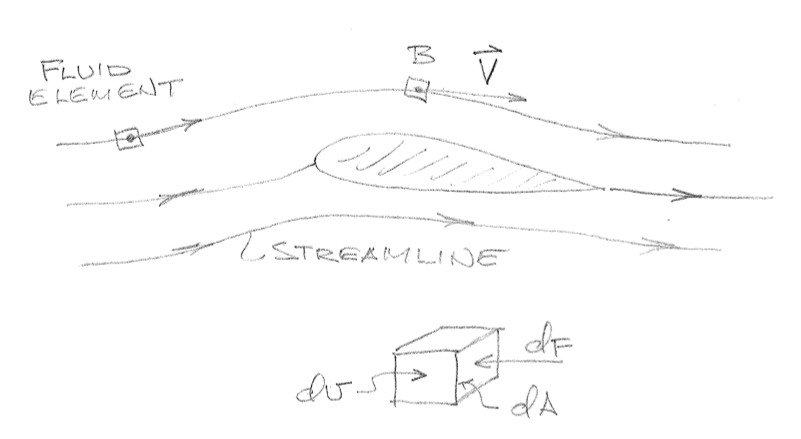
\includegraphics[width=0.7\linewidth]{Figures/pg1_1.png}
    \caption{Fluid Element and Streamline}
    \label{fig:pg1_1}
\end{figure}

\begin{table}[ht]
    \centering
    % arraystretch widens the space between each row
    \renewcommand{\arraystretch}{1.5}
    \caption{Aerodynamic Variable Definitions}
    \begin{tabular}{l|rcl}
         Pressure & p &=& $\lim\limits_{d\Delta \to 0} \frac{dF}{dA}$, a scalar quantity\\
         Density & $\rho$ &=& $\lim\limits_{dv\to 0} \frac{dw}{dv}$, a scalar quantity\\
         Temperature (Kinetic Energy) & $KE$ &=& $\frac{3}{2}kT$, scalar (k = Boltzmann Const.)\\
         Perfect Gas Law & $p$ &=& $\rho RT$ (R = Gas Const.)\\
         Velocity & $\vec{V}$ &=& Velocity of element B, a vector\\
         
    \end{tabular}
    \label{tab:my_label}
\end{table}

\subsection{Aerodynamic Forces and Moments}
\begin{figure}[ht]
    \centering
    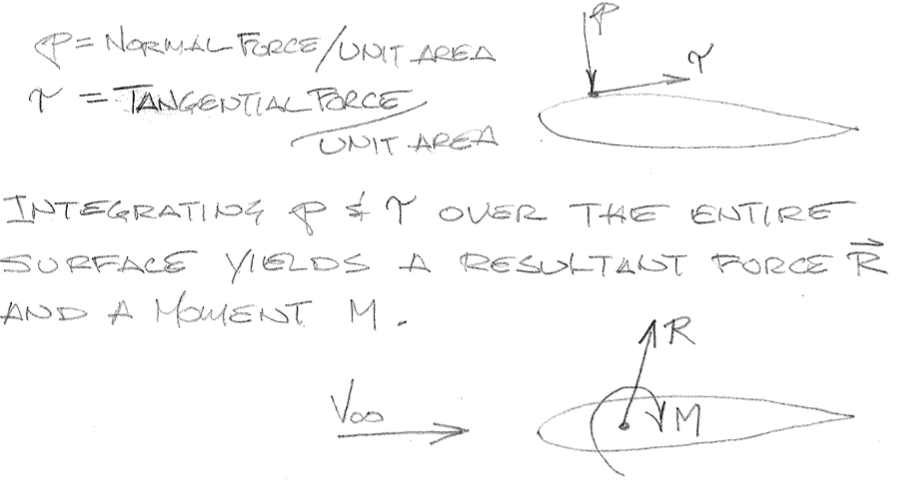
\includegraphics[width=0.9\linewidth]{Figures/p2_1.png}
    \caption{Force on Airfoil}
    \label{fig:p2_1}
\end{figure}

\begin{figure}[ht]
    \centering
    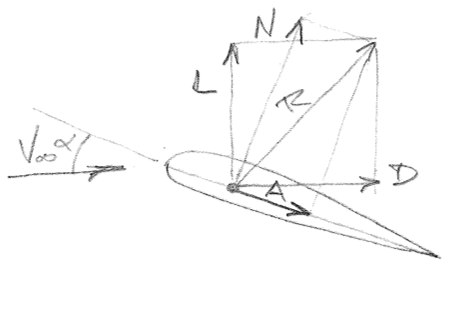
\includegraphics[width=0.5\linewidth]{Figures/p2_2.png}
    \caption{Force Definitions}
    \label{fig:p2_2}
\end{figure}

Figure \ref{fig:p2_1} and \ref{fig:p2_2}: The force on a unit area of the airfoil is $P$, the normal force and $\tau$, the tangential force. Integrating $P$ and $\tau$ over the entire surface yields a resultant force $\vec{R}$ and a moment $M$.

% this should go in another table, tables are useful
\begin{table}[ht]
\centering
\renewcommand{\arraystretch}{1.3}
\caption{Variable Definitions for Airfoil}
\begin{tabular}{rcl}
\hline
Lift &=& force perpendicular to $\vec{V}_\infty$.\\
Drag &=& Force parallel to $\vec{V}_\infty$\\
Chord &=& Max length line from trailing edge to leading edge = c\\
Normal Force &=& Force perpendicular to C=N\\
Chord Force &=& Force parallel to C=A\\
$L$ &=& $N\cos\alpha - A\sin\alpha$\\
$D$ &=& $N\sin\alpha + A\cos\alpha$\\
Dynamic Pressure &=& $q=\frac{1}{2}\rho_\infty V_\infty ^2$\\
Reference Area &=& S (typically wing area)\\
Reference Length &=& C (typically wing chord)\\
\hline
\end{tabular}

\end{table}

\subsubsection{Coefficients for 2D and 3D bodies}

% Notice this is a different type of table.
% It is actually a large equation array
% The equation array comes from the amsmath package and is extremely useful
\begin{equation}
    \begin{array}{lrcl}
         \text{Lift Coefficient} & C_L &=& L/(q_\infty S)\\
         \text{Drag Coefficient} & C_D &=& D/(q_\infty S)\\
         \text{Moment Coefficient} & C_M &=& M/(q_\infty Sc)\\
    \end{array}
\end{equation}

For 2D airfoils the area $S=C\cdot 1$. Define:
% Note that equation* is unnumbered and equation is numbered
\begin{equation}
    C_l \ L'/(q_\infty c),\quad C_d = D'/(q_\infty c),\quad C_m \ M'/(q_\infty c^2)
\end{equation}
$L',\ D',\ M'$ are defined per unit span. Define "Force" coefficients as:
\begin{equation}
    C_p = \frac{p-p_\infty}{q_\infty} = \text{Pressure Coefficient}
\end{equation}
\begin{equation}
    C_f = \frac{\tau}{q_\infty} = \text{Skin Friction Coefficient}
\end{equation}
where $p_\infty$ is the free stream static pressure and $q_\infty = \frac{1}{2}\rho_\infty V_\infty ^2$.

\subsection{Integration of P and T on a 2D Body}
\begin{figure}[ht]
    \centering
    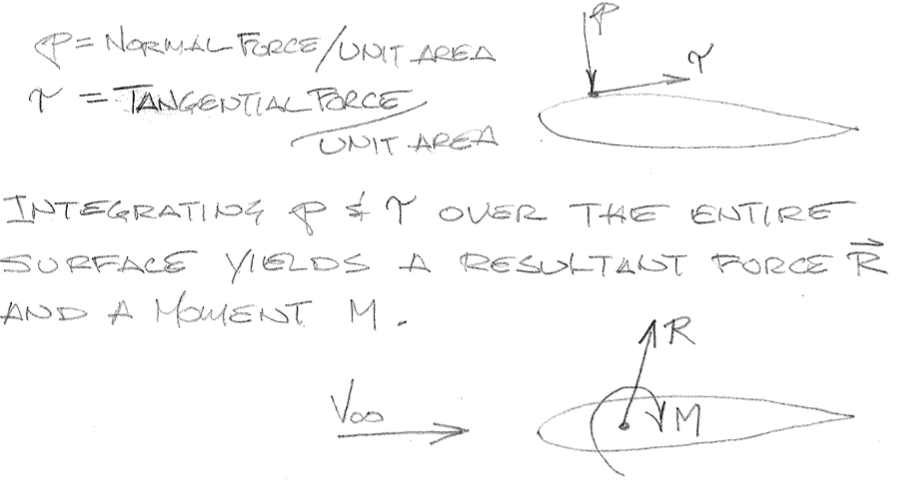
\includegraphics[width=0.6\linewidth]{Figures/p2_1.png}
    \caption{Force on Airfoil Surface and Resulting Force R and Moment M}
    \label{fig:p3_1}
\end{figure}

Along the upper surface of the airfoil (subscript u):
\begin{equation*}
    \begin{array}{rcl}
         dN_u &=& -P_u ds_u\cos\theta - T_u ds_u \sin\theta \\
         dA_u &=& -P_uds_u \sin\theta + T_uds_u \cos\theta \\
    \end{array}
\end{equation*}
Along the lower surface of the airfoil (subscript l):
\begin{equation*}
    \begin{array}{rcl}
         dN_l &=& P_l ds_l\cos\theta - T_l ds_l \sin\theta \\
         dA_l &=& P_lds_l \sin\theta + T_lds_l \cos\theta \\
    \end{array}
\end{equation*}
For the moment about the leading edge (LE), clockwise is \textbf{positive}.
\begin{equation*}
    \begin{array}{rcl}
    dM_u &=& (P_u\cos\theta + T_u\sin\theta)xds_u + (-P_u\sin\theta + T_u\cos\theta)yds_u \\
    dM_l &=& (-P_l\cos\theta + T_l\sin\theta )xds_l + (P_l \sin\theta + T_l\cos\theta)yds_l \\
    \end{array}
\end{equation*}
For the surface element $ds$, $dx = ds \cos\theta $ and $dy = -ds\sin\theta$.\\
$\theta$ is measured clockwise positive from $dx.\ ds$ is the surface of the airfoil.
   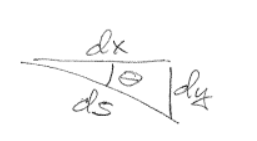
\includegraphics[width=30mm]{Figures/surface_element.PNG}
% this is an inline image

\begin{equation*}
    \renewcommand{\arraystretch}{1.75}
    \begin{array}{lrcl}
         & dN_u &=& -P_udx_u + T_u dy_u \\
         \text{Convert to dx because we DO NOT KNOW dy} & dN_u &=& (-P_u + T_u \frac{dy_u}{dx}) dx \\
         \text{Same for lower side} & dN_l &=& p_ldx_l + T_ldy_l \\
         & dN_l &=& (P_l + T_l \frac{dy_l}{dx})dx \\
         \text{Integrate to get N, the normal force} &
         N &=& \int_{LE}^{TE}(dN_u + dN_l) \\
         \text{Separate T and P terms} & N &=& \int_{LE}^{TE}(P_l - P_u)dx + \int_{LE}^{TE}(T_u\frac{dy_u}{dx} + T_l\frac{dy_l}{dx})dx \\
         \text{Use } C_n \ \frac{N}{q_\infty c},\ C_p,\ C_f \text{ (convert to dimensionless)} &
         C_n &=& \int_0^1(C_{p_l} - C_{p_u})d(\frac{x}{c}) + \int_0^1(C_{f_u}\frac{dy_u}{dx} + C_{f_l}\frac{dy_l}{dx})d(\frac{x}{c}) \\
         
         \text{Similarly for A and M} &
         C_a &=& \int_0^1(C_{p_u}\frac{dy_u}{dx} - C_{p_l}\frac{dy_l}{dx})d(\frac{x}{c}) + \int_0^1(C_{f_u} + C_{f_l})d(\frac{x}{c}) \\
         
         \text{For the moment about the leading edge:} & C_{M_{LE}} &=& \int_0^1(C_{p_u} - C_{p_l})\frac{x}{c}d(\frac{x}{c}) - \int_0^1 (C_{f_u}\frac{dy+u}{dx} + C_{f_l}\frac{dy_l}{dx}) \frac{x}{c}d(\frac{x}{c}) \\
         & &+& \int_0^1(C_{p_u}\frac{dy_u}{dx} + C_{f_u})(\frac{y+u}{x})d(\frac{x}{c}) \\
         & &+& \int_0^1 (-C_{p_l}\frac{dy_l}{dx} + C_{f_l})(\frac{y_l}{x})d(\frac{x}{c}) \\
    \end{array}
\end{equation*}

\subsection{Center of Pressure}
\begin{figure}[ht]
    \centering
    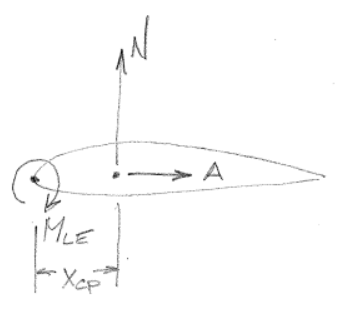
\includegraphics[width=0.3\linewidth]{Figures/center_of_pressure.PNG}
    \caption{Center of Pressure and Moment at Leading Edge}
    \label{fig:center_of_pressure}
\end{figure}

Based on the definition of normal force N and chord force A, in Figure \ref{fig:center_of_pressure}:
\begin{equation}
    X_{CP} = -\frac{M_{LE}}{N}
\end{equation}
For small $\alpha$, N is close to L. So
\begin{equation}
    X_{CP} = -\frac{M_{LE}}{L}
\end{equation}

In Figure \ref{fig:center_of_pressure2} the net moment is the same. (The moment is taken about different points but must always sum to the same value.)

\begin{figure}[ht]
    \centering
    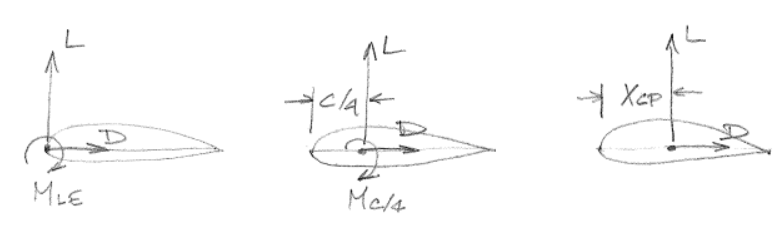
\includegraphics[width=0.9\linewidth]{Figures/center_of_pressure_2.PNG}
    \caption{Center of Pressure and Moment in 3 Configurations}
    \label{fig:center_of_pressure2}
\end{figure}

\begin{equation}
    M_{LE} = -\frac{c}{4}L + M_{c/4} = -X_{CP}L
\end{equation}

% PRAGMA MARK NEW SECTION, page 8
\section{Drag, Fluid Statics, Dimensional Analysis}
\subsection{Comments on Drag}
Recall the relation for $C_a$ (Equation \ref{eq:C_a_integral}). The first term (containing $C_p$) is the pressure drag and the second ($C_f$) is the skin friction drag. The amount of each varies with the object's geometry. In Figure \ref{fig:drag_comparison} the drag of the streamlined body is the SAME as the drag on a cylinder $1/10^{th}$ its diameter.
\begin{equation}
    C_a = \int_0^1(C_{p_u}\frac{dy_u}{dx} - C_{p_l}\frac{dy_l}{dx})d(\frac{x}{c}) + \int_0^1(C_{f_u} + C_{f_l})d(\frac{x}{c})
    \label{eq:C_a_integral}
\end{equation}

\begin{figure}[ht]
    \centering
    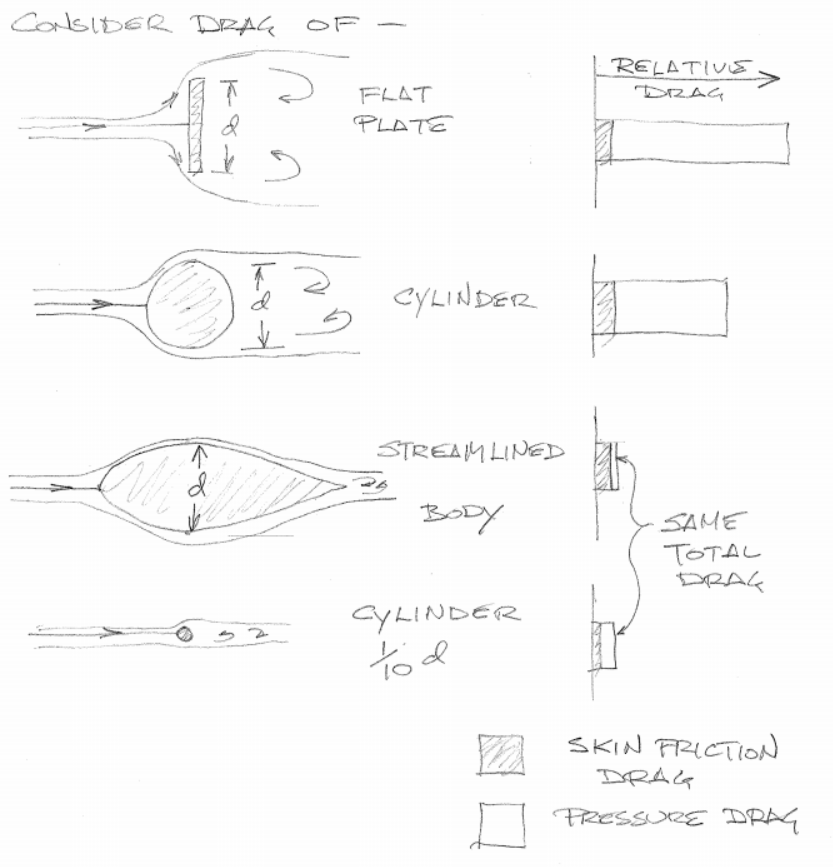
\includegraphics[width=0.8\linewidth]{Figures/drag_comparison.PNG}
    \caption{Drag Comparison for Plate, Cylinder, Streamlined Body}
    \label{fig:drag_comparison}
\end{figure}

\subsection{Fluid Statics: Buoyancy}
\begin{figure}[ht]
    \centering
    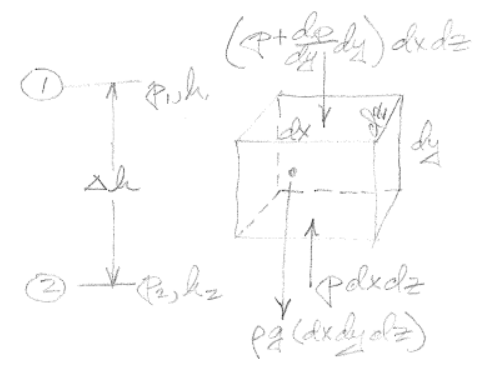
\includegraphics[width=0.5\linewidth]{Figures/staticElement.PNG}
    \caption{An element in a stagnant fluid}
    \label{fig:staticElement}
\end{figure}
Consider a static fluid (Figure \ref{fig:staticElement}).
\begin{align*}
    \text{Net pressure force} \quad&= pdxdz - (p + \frac{dp}{dy} dy)\ dx\ dz\\
    &= -\frac{dp}{dy}\ dx\ dy\ dz\\
    \text{Gravity force} \quad&= -\rho  g\ dx\ dy\ dz\\
    \text{static} \quad&= \sum F_y = -\frac{dp}{dy}\ dx\ dy\ dz - \rho g\ dx\ dy\ dz = 0\\
    \text{Hydrostatic equation} \quad&= dp = -\rho g dy\\
    \text{For } \rho = const \quad &= \int_{p1}^{p2} dp = -\rho g \int_{h1}^{h2} dy\\
    &= p_2 - p_1 = -\rho g(h_2 - h_1 = \rho g \Delta h\\
    \text{or} \quad&= p + \rho gh = const
\end{align*}

\begin{figure}[ht]
    \centering
    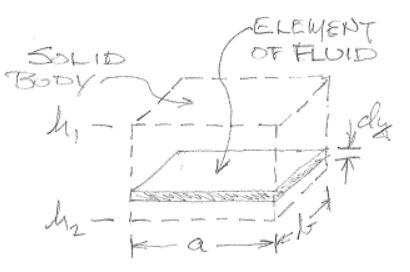
\includegraphics[width=0.4\linewidth]{Figures/bodyInFluid.PNG}
    \caption{A body immersed in a static fluid}
    \label{fig:bodyInFluid}
\end{figure}
Consider a solid body immersed in a fluid (Figure \ref{fig:bodyInFluid}). The vertical force on the body is $F=(p_2-p_1)ab$. Integrating the hydrostatic equation:
\begin{gather*}
    p_2-p_1 = \int_{p1}^{p2} dp = -\int_{h1}^{h2} \rho g dy = \int_{h2}^{h1} \rho g dy\\
    F = ab\int_{h2}^{h1} \rho g dy
\end{gather*}
The \textbf{weight} of the column of fluid displaced by the solid body is
\begin{equation*}
    W = ab \int_{h2}^{h1} \rho g dy
\end{equation*}
The buoyancy force on the body = the weight of the fluid displaced by the body (Archimedes Principle).\\
\textbf{Note: $\rho$ has not been assumed constant.}

\subsection{Dimensional Analysis}
The aero force is $R=f(\rho_\infty,\ V_\infty,\ e,\ \mu_\infty,\ a_\infty)$. All variables can be expressed in terms of \textbf{fundamental dimensions} m, l, and t. Then the number of fundamental dimensions $K=3$.\\
Given a physical relation $f_1(P_1,\ P_2,...,P_N) = 0$ this can be presented as a relation with $n-K$ dimensionless products $\Pi's,\ f_2(\Pi_1,\ \Pi_2,...,\Pi_{N-K})=0$ where each $\Pi$ is a product of the K fundamental dimensions.
\begin{center}
    $\Pi_1 = f_3(P_1,\ P_2,...,\ P_K,\ P_{K+1})$\\
    $\Pi_1 = f_4(P_1,\ P_2,...,\ P_K,\ P_{K+2})$\\
    ...\\
    $\Pi_{N-K} = f_3(P_1,\ P_2,...,\ P_K,\ P_{N})$
\end{center}
The dependent variable R should appear in only one of the $\Pi$ terms.

\paragraph*{} Rewrite $R=f(...)$ as
\begin{center}
    $g(R,\ \rho_\infty,\ V_\infty,\ c,\ \mu_\infty,\ a_\infty)$\\
    $[R] = mlt^{-2}$\\
    $[\rho_\infty] = ml^{-3}$\\
    $[V_\infty] = lt^{-1}$\\
    $[c] = l$\\
    $[\mu_\infty] = ml^{-1}t^1$\\
    $[a_\infty] = lt^{-1}$
\end{center}
Here, $N-K=G-3=3$.
\begin{center}
    $f_2(\Pi_1,\ \Pi_2,\ \Pi_3) = 0$\\
    $\Pi_1 = f_2(\rho_\infty,\ V_\infty,\ c,\ R)$\\
    $\Pi_2 = f_3(\rho_\infty,\ V_\infty,\ c,\ \mu_\infty)$\\
    $\Pi_3 = f_2(\rho_\infty,\ V_\infty,\ c,\ a_\infty)$\\
    $\Pi_1 = \rho\infty^d V_\infty^b c^e R$\\
    $[\Pi_1] = (ml^{-3})^d(lt^{-1})^b(l)^e(mlt^{-2})$
\end{center}
For $\Pi$ to be dimensionless the exponents of m, l, and t must each sum to zero.
\begin{align*}
    m:\ & d + 1 = 0\\
    l:\ & -3d + b + e + 1 = 0\\
    t:\ & -b -2 = 0\\
    & d=-1,\quad b=-2,\quad e=-2\\
    & \Pi_1 = R\rho_\infty^{-1}V_\infty^{-2}C^{-2}\\
    & \frac{R}{\rho_\infty V_\infty^2 c^2} \rightarrow C_l = \frac{W/s}{\frac{1}{2}\rho_\infty V_\infty^2}\\
    \text{Similarly} \quad& \Pi_2 = \frac{\rho_\infty V_\infty c}{\mu_\infty} = RM
    \quad\text{and}\quad
    \Pi_3 = \frac{V_\infty}{a_\infty} = M\\
    \text{or} \quad& f_2\Big(\frac{R}{\frac{1}{2}\rho_\infty V_\infty^2 S},\ \frac{\rho_\infty V_\infty c)}{\mu_\infty},\ \frac{V_\infty}{a_\infty}\Big) = 0\\
    & C_L = f_6(RN, M_\infty)
\end{align*}

\subsection{Vector Relations}
Need to know addition: $\vec{A} + \vec{B} = \vec{C}$ and subtraction.
\subsubsection{Dot Product} $\vec{A} \bullet \vec{B} = |A||B|\cos\theta$ is a SCALAR. We can think of it as $|A|(\text{component of } \vec{B}\ || \text{ to } \vec{A})$.
\subsubsection{Cross Product} $\vec{A} \times \vec{B} = (|A||B|\sin\theta)\vec{e} = \vec{G}$. The unit vector $\vec{e}$ is perpendicular to the plane formed by $\vec{A}$ and $\vec{B}$ using the \textbf{right-hand-rule}.
\subsubsection{Orthogonal Coordinate System}
\begin{equation}
    \vec{r} = x\vec{i} + y\vec{j} + z\vec{k} \quad \text{and} \quad |r| = (x^2 + y^2 + z^2)^{1/2}
\end{equation}

\subsubsection{Scalar and Vector Fields}
See Table \ref{tab:ScalarVectorFields}.
\begin{table}[ht]
\centering\caption{Scalar and Vector Fields}
    \begin{tabular}{rcl}
    \hline
         P &=& P(x, y, z, t) \\
         $\rho$ &=& $\rho(x, y, z, t)$ \\
         T &=& T(x, y, z, t) \\
         $\vec{V}$ &=& $V_x\vec{i} + V_y\vec{j} + V_z\vec{k}$ \\
         $V_x$ &=& $V_x(x, y, z, t)$ \\
         $V_y$ &=& $V_y(x, y, z, t)$ \\
         $V_z$ &=& $V_z(x, y, z, t)$ \\
         \hline
    \end{tabular}
    \label{tab:ScalarVectorFields}
\end{table}

\subsubsection{Gradient of a Scalar Field} Consider a 2D pressure field $P_1 > P_2 > P_3$ where $P=P(x, y)$. (Figure \ref{fig:gradient_field}) Then the gradient is:
\begin{equation}
    \vec{\nabla}p = \frac{\partial p}{\partial x}\vec{i} + \frac{\partial p}{\partial y}\vec{j}
\end{equation}

\begin{figure}[ht]
    \centering
    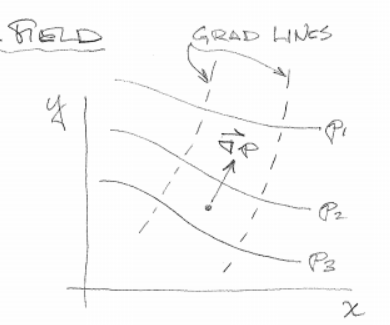
\includegraphics[width=0.3\linewidth]{Figures/gradient_field.PNG}
    \caption{Gradient field with constant-pressure lines}
    \label{fig:gradient_field}
\end{figure}

$|\vec{\nabla}|$ represents the magnitude of the maximum rate of change of P per unit length.\\
The direction of $\vec{\nabla}p$ is the direction of the max rate of change of P. Generally:
\begin{equation}
    \gradient P = \frac{\partial p}{\partial x}\vec{i} + \frac{\partial p}{\partial y}\vec{j} + \frac{\partial p}{\partial z}\vec{k}
\end{equation}
For this rate of change of P in an arbitrary direction $\vec{S}$, where $\vec{n}$ is the unit vector in that direction
\begin{equation}
    \frac{dp}{ds} = \gradient p \cdot \vec{h} \quad \text{and} \quad \frac{dp}{ds} = |\gradient p| \cos\theta
\end{equation}

\begin{figure}[ht]
    \centering
    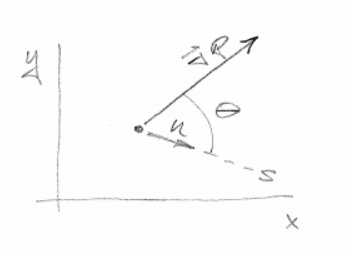
\includegraphics[width=0.25\linewidth]{Figures/gradient_2.PNG}
    \caption{Vectors P and n}
    \label{fig:gradient_2}
\end{figure}

\subsubsection{Divergence of a Vector Field}
Consider a vector field where $\vec{V}(x, y, z)$ is the flow velocity.\\
Next consider a small fluid element of \textbf{fixed mass} moving along a streamline with velocity $\vec{V}$. The rate of change of the volume of the fluid element is given by the \textbf{divergence of $\vec{V}$} (Equation \ref{eq:Divergence}).
\begin{equation}
    \gradient \bullet \vec{V} = \frac{\partial V_x}{\partial x} + \frac{\partial V_y}{\partial y} + \frac{\partial V_z}{\partial z}
    \label{eq:Divergence}
\end{equation}

\subsubsection{Curl of a Vector Field}
Again, consider a velocity field and a fluid element with velocity $\vec{V}$. Said fluid element may be rotating with angular velocity $\vec{\omega}$. It can be shown that $\vec{\omega} = 1/2 \gradient \times \vec{V}$ where curl(V) is given by Equation \ref{eq:Curl}.
\begin{equation}
    \text{Curl } \vec{V} = \gradient \times \vec{V} \ \Big( \frac{\partial V_z}{\partial y} - \frac{\partial V_y}{\partial z} \Big) \vec{i} + 
    \Big( \frac{\partial V_x}{\partial z} - \frac{\partial V_z}{\partial x} \Big) \vec{j} +
    \Big( \frac{\partial V_y}{\partial x} - \frac{\partial V_x}{\partial y} \Big) \vec{k}
    \label{eq:Curl}
\end{equation}

% PRAGMA MARK NEW SECTION, page 17
\section{Integrals}
\subsection{Line Integrals}
\begin{figure}[ht]
    \centering
    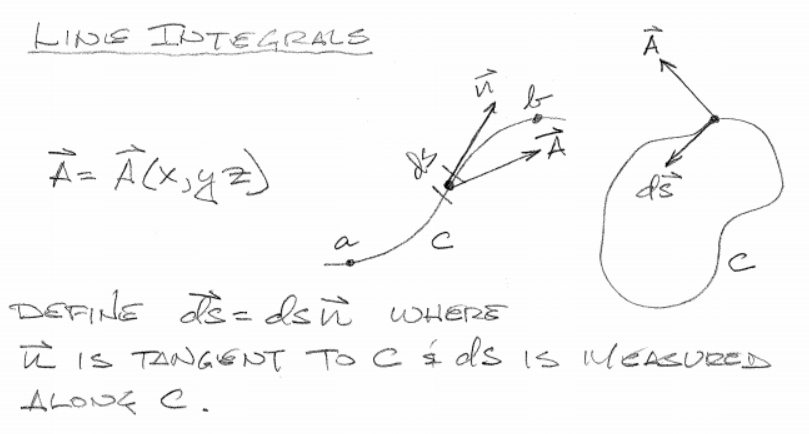
\includegraphics[width=0.7\textwidth]{Figures/line_integrals.PNG}
    \caption{Line Integral on Open and Closed Curve}
    \label{fig:line_integral}
\end{figure}

A line integral integrates a vector function along an open or closed curve.\\
Define $\vec{ds} = ds\vec{n}$ where $\vec{n}$ is tangent to the curve C and $ds$ is measured along C. (Figure \ref{fig:line_integral}). The line integral of a vector  $\vec{A}$ along C is Equation \ref{eq:line_integral} where \textbf{counterclockwise along C is positive.}

\begin{equation}
    \int_a^b\vec{A}\bullet \vec{ds}\quad \text{If C is closed:} \quad \oint_C \vec{A}\bullet \vec{ds}
    \label{eq:line_integral}
\end{equation}

\subsection{Surface Integrals}
\begin{figure}[ht]
    \centering
    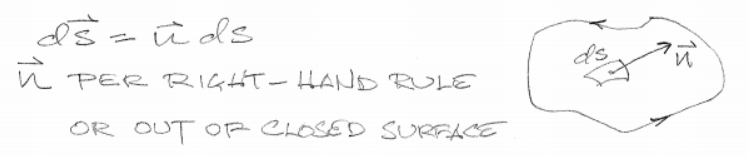
\includegraphics[width=0.7\textwidth]{Figures/surface_integrals.PNG}
    \caption{Surface Integral on Closed Surface}
    \label{fig:surface_integral}
\end{figure}

Again, $d\vec{s} \ \vec{u}ds.\ \vec{u}$ is per right-hand-rule or out of the closed surface. There are three possibilities for surface integrals (Equation \ref{eq:surface_integral}).
\begin{equation}
    \begin{array}{lc}
         \text{Scalar function, vector result:} & \oiint_S p d\vec{s} \\
         \text{Vector function, scalar result:} & \oiint_S \vec{A}\bullet\vec{ds} \\
         \text{Vector function, vector result:} & \oiint_S \vec{A} \times \vec{ds} \\
    \end{array}
    \label{eq:surface_integral}
\end{equation}

\subsection{Volume Integrals}
\begin{equation}
    \iiint_V \rho dv\ \text{Scalar result} \quad \iiint_V \vec{A}dv\ \text{Vector result}
\end{equation}
\textit{Note: These should be closed integrals but due to a collision between packages it became difficult to bring in the closed triple integral symbol.}

\subsubsection{Stokes Theorem}
Converts between a line integral on a closed curve and a surface integral for the surface the curve encloses.
\begin{equation}
    \oint_C \vec{A} \bullet \vec{ds} = \oiint_S (\gradient \times \vec{A})\vec{ds}
\end{equation}
\subsubsection{Divergence Theorem}
Converts between a surface integral and a volume integral for a vector integrand.
\begin{equation}
    \oiint_S\vec{A}\bullet \vec{ds} = \iiint_V (\gradient \bullet \vec{A})dV
\end{equation}
\subsubsection{Gradient Theorem}
Converts between a surface integral and a volume integral for a scalar integrand.
\begin{equation}
    \oiint_S p\vec{ds} = \iiint_V \gradient p dV
\end{equation}

% PRAGMA MARK NEW SECTION, page 19
\section{Continuity Equation}

\begin{figure}
    \centering
    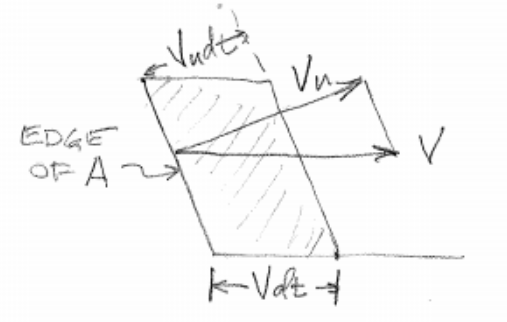
\includegraphics[width=0.4\linewidth]{Figures/continuity_A}
    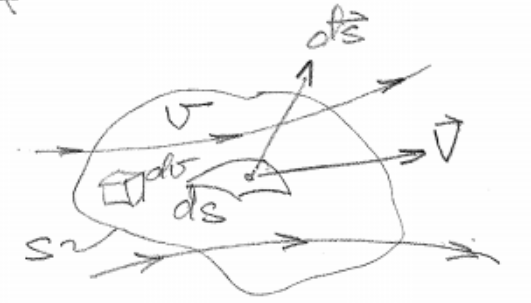
\includegraphics[width=0.4\linewidth]{Figures/continuity_CV}
    \caption{Continuity for an area A and a fixed control volume}
    \label{fig:continuity_CV}
\end{figure}

Consider an area A in a fluid flow field (Figure \ref{fig:continuity_CV}). The \textbf{volume} is $(V_udt) A$. The \textbf{mass} is $\rho V_u dt A$ and the mass flow rate $\dot{m} = \rho V_u A$.\\
Consider a fixed control volume (Figure \ref{fig:continuity_CV}). The mass flow across $ds$ is
\begin{equation*}
\rho V_u ds = \rho \vec{V} \bullet \vec{ds}
\end{equation*}
\begin{equation*}
    \text{The net mass flow out of the volume V is} \quad B=\oiint_S \rho \vec{V} \bullet \vec{ds}
\end{equation*}
\begin{equation*}
    \text{The total mass in V is} \quad V = \iiint_V \rho dV
\end{equation*}
The rate of decrease (negative) of mass is the differential:
\begin{equation*}
    -\frac{\partial}{\partial t} \iiint_V \rho dV = c
\end{equation*}
For continuity, $B=c$ (the net mass flow OUT equals the rate of decrease of mass in the control volume). Then write $B-c = 0$:
\begin{equation}
   \boxed{ \oiint_S \rho \vec{V} \bullet \vec{ds} +\frac{\partial}{\partial t} \iiint_V \rho dV = 0 }
\end{equation}

\begin{equation*}
    \renewcommand{\arraystretch}{1.5}
    \begin{array}{lrcl}
         \text{Since V is fixed in space (fixed control volume)} &
        \frac{\partial}{\partial t} \iiint_V \rho dV &=& \iiint_V \frac{\partial \rho}{\partial t} dV \\
        
        \text{From the Divergence Theorem} &
        \oiint_S (\rho \vec{V}) \bullet \vec{ds} &=& \iiint_V \gradient \bullet (\rho \vec{V}) dV \\
        
        \text{Rewrite line 1 as} &
        \iiint_V \frac{\partial \rho}{\partial t} dV + \iiint_V \gradient \bullet (\rho \vec{V}) dV \\
        
        \text{Combine integrals} &
        \iint_V \Big[ \frac{\partial \rho}{\partial t} + \gradient \bullet (\rho \vec{V}) \Big] dV &=& 0 \\
        
        \text{V is defined as arbitrary (switch to differential form)} &
        \frac{\partial \rho}{\partial t} + \gradient \bullet (\rho \vec{V}) &=& 0 \\
        
        \text{In general, apply} & \rho &=& \rho(x, y, z, t) \\
        \text{For steady flow} & \rho &=& \rho(x, y, z) \\
        \text{This yields} & \oiint_C \rho \vec{V} \bullet \vec{ds} &=& 0 \\
        \text{and} & \nabla \bullet (\rho \vec{V}) &=& 0

    \end{array}
\end{equation*}

% PRAGMA MARK NEW SECTION, page 21
\section{Momentum Equation}
\begin{figure}
    \centering
    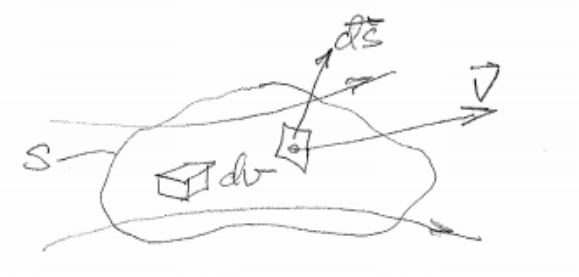
\includegraphics[width=0.4\linewidth]{Figures/momentum_CV.PNG}
    \caption{Momentum through an Arbitrary Control Volume}
    \label{fig:momentum_CV}
\end{figure}

Again, consider a control volume fixed in space (Figure \ref{fig:momentum_CV}).
\begin{equation*}
    \renewcommand{\arraystretch}{1.5}
    \begin{array}{rcl}
         \text{Body Force} &=& \iiint_V \rho \vec{f} dV\ \vec{f} = \frac{\text{Body Force}}{\text{Unit Mass}} \\
         
         \text{Pressure Force} &=& -\oiint_S p\vec{ds}\ \text{Due to force opposite } \vec{ds} \\
         
         \text{Viscous Force} &=& \vec{F}_{vis}\ \text{Total on surface S} \\
         
         \text{Momentum Flux out of V} &=& \oiint_S (\rho \vec{V} \bullet \vec{ds}) \vec{V} \\
         
         \text{Momentum in V} &=& \iiint_V \rho \vec{V} dV \\
         
         \text{Rate of change of momentum} &=& \deldelt \volumeint \rho \vec{V} dV\ \text{is 0 if steady} \\
         
         \text{Newton's 2nd Law} & & \frac{d}{dt}(m\vec{V}) = \vec{F} \\
    \end{array}
\end{equation*}

\begin{equation}
    \boxed{ \deldelt \volumeint \rho \vec{V} dV + \oiint_S (\rho \vec{V} \bullet \vec{ds}) \vec{V} = -\oiint_S p \vec{ds} + \volumeint \rho \vec{f} dV + \vec{F_v} }
    \label{eq:Momentum}
\end{equation}

\begin{equation*}
    \text{Since V is fixed: } \deldelt \volumeint \rho \vec{V} dV = \volumeint \deldelt (\rho \vec{V}) dV
\end{equation*}
\begin{equation*}
    \text{Gradient Theorem: } -\oiint_{ds} p\vec{ds} = -\volumeint \gradient p dV
\end{equation*}

The integral form of the momentum equation (\ref{eq:Momentum}) is a vector equation which can be written as 3 scalar equations. Define: $\vec{V} = u\vec{i} + v\vec{j} + w\vec{k}$. Then the x-component of momentum is Equation \ref{eq:xmomentum}) where $\rho \vec{V} \bullet \vec{ds}$ is a scalar.
\begin{equation}
    \volumeint \deldelt (\rho u) dV + \iint_S (\rho \vec{V} \bullet \vec{ds})u = -\volumeint \frac{\partial p}{\partial x} dV + \volumeint \rho f_x dV + F_v|_x
    \label{eq:xmomentum}
\end{equation}

We apply the divergence theorem, converting the surface integral to a volume integral.
\begin{equation}
    \oiint_S (\rho \vec{V} \bullet\vec{ds}) u = \oiint_S (\rho u\vec{V}) \bullet\vec{ds} = \volumeint \gradient \bullet (\rho u \vec{V}) dV
\end{equation}
Now all terms can be combined in a single volume integral.
\begin{equation}
    \volumeint\Big[ \deldelt (\rho u) + \gradient \bullet(\rho u \vec{V}) + \frac{\partial p}{\partial x} - \rho f_x -F_{v_x} \Big] dV = 0
\end{equation}

Since V is arbitrary, switch to differential form
\begin{equation}
    \deldelt (\rho u) + \gradient \bullet(\rho u \vec{V}) = -\frac{\partial p}{\partial x} + \rho f_x + F_{v_x}
\end{equation}
Similar equations replacing x with y and z apply to the other dimensions.
\subsection{Steady Inviscid Flow}
For steady inviscid flow with no body force:
\begin{equation}
    \oiint_S (\rho \vec{V} \bullet \vec{ds}) \vec{V} = -\oiint_S p \vec{ds}
\end{equation}

And the 3 components are Equation \ref{eq:euler_eqs}. These are the \textbf{Euler Equations}.
\begin{equation}
    \begin{array}{rcl}
         \gradient \bullet(\rho u \vec{V}) &=& -\frac{\partial p}{\partial x} \\
         \gradient \bullet(\rho v \vec{V}) &=& -\frac{\partial p}{\partial y} \\
         \gradient \bullet(\rho w \vec{V}) &=& -\frac{\partial p}{\partial z} \\
    \end{array}
    \label{eq:euler_eqs}
\end{equation}

% PRAGMA MARK NEW SECTION, page 24
% TRANSITION TO AIRFOIL STUFF
\section{Example: Airfoil Drag}
\begin{figure}[ht]
    \centering
    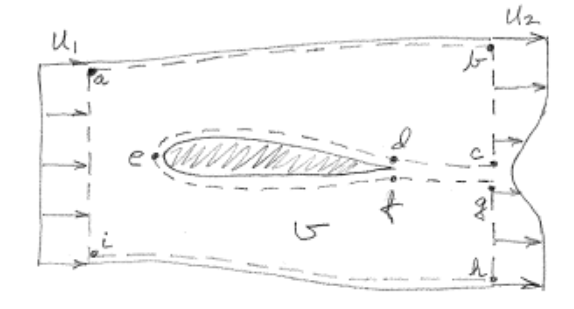
\includegraphics[width=0.7\linewidth]{Figures/airfoil_drag.PNG}
    \caption{Example: Drag on an Airfoil in a Control Volume}
    \label{fig:airfoil_drag}
\end{figure}

Consider a 2D wing in a uniform onset flow. Draw a control volume such that:
\begin{enumerate}
\item abhi is far from the wing, then $P=P_\infty$ on abhi
\item $u_1$ and $u_2$ are parallel to x
\end{enumerate}
List the surface forces on v:
\begin{enumerate}
    \item On the boundary abhi, shear forces are zero, and the pressure force is
\begin{equation*}
    -\iint_{abhi} p \vec{ds}
\end{equation*}
\item The surface forces on cd and fg cancel
\item Let $\vec{R}$ be the net aerodynamic force on the wing. Then $-\vec{R}$ is the surface force on def
\end{enumerate}

The total surface force on v is
\begin{equation*}
-\oiint_{abhi} p \vec{ds} - \vec{R}
\end{equation*}
Writing the integral form of the momentum equation:
\begin{equation*}
    \deldelt \volumeint\rho \vec{V} dV + \oiint_S (\rho \vec{V} \bullet \vec{ds}) \vec{V} = -\oiint_{abhi} p\vec{ds} - \vec{R}
\end{equation*}

Since the surface force above is the total force (there are no body forces) on the fluid passing through V, and V is chosen to be large enough that $P=P_\infty$ everywhere on abhi:
\begin{equation*}
    \iint_{abhi} p \vec{ds} = 0
\end{equation*}

Assuming steady flow, $\deldelt(~) = 0$ and the momentum equation reduces to
\begin{equation*}
    \oiint_S (\rho \vec{V} \bullet\vec{ds})\vec{V} = -\vec{R}
\end{equation*}

Or in terms of the aerodynamic force $\vec{R}$ \textbf{on} the wing
\begin{equation*}
    \vec{R} = \oiint_S (\rho \vec{V} \bullet\vec{ds}) \vec{V}
\end{equation*}
The x-component gives the drag
\begin{equation*}
    D = \oiint_S (\rho \vec{V} \bullet\vec{ds}) u
\end{equation*}
\begin{enumerate}
    \item Since ab, hi, and def are streamlines, $\vec{V}$ is perpendicular to $\vec{ds}$ and $\vec{V} \bullet \vec{ds} = 0$
    \item cd and fg are adjacent, hence the mass flux $\rho \vec{V}$ cancels
    \item The only contribution to D comes from sections ai and bh
\end{enumerate}
\begin{equation*}
    D = -\int_i^a\rho_1 u_1^2 dy + \int_h^b \rho_2 u_2^2 dy
\end{equation*}
(The minus on ai is due to $\vec{V}$ being inward on $\vec{ds}$ along ai.)\\
Applying the continuity equation, which is
\begin{equation*}
    -\int_i^a \rho_u u_1 dy + \int_h^b \rho_2 u_2 dy = 0
\end{equation*}
Multiply the continuity equation by $u_1$, a constant. Then
\begin{equation*}
    \int_c^a \rho_1 u_1^2 dy = \int_h^b \rho_2 u_2 u_1 dy
\end{equation*}
Substitute in the drag equation. The final result is Equation \ref{eq:drag_u1_u2}.
\begin{equation}
    D = \int_h^b \rho_2 u_2(u_1-u_2) dy
    \label{eq:drag_u1_u2}
\end{equation}
In a similar fashion, lift on a wing in a wind tunnel can be obtained by measuring the pressure distribution on the floor and ceiling of the test section. (In this case, ab and hi are not far enough away such that $p=p_\infty$ and they are not natural streamlines.)

\subsection{Energy Equation}
Consider a fixed amount of water within a closed boundary. This water is the \textbf{system}. The region outside of the system is the \textbf{surroundings}.\\
$\delta q$ = heat added to the system from the surroundings\\
$\delta w$ = work done on the system by the surroundings\\
$\delta e$ = change in internal energy of the system due to $\delta q, \delta w$.\\
For conservation of energy:
\begin{equation*}
    \delta q + \delta w = \delta e
\end{equation*}
This is the \textbf{First Law of Thermodynamics.}

\begin{figure}
    \centering
    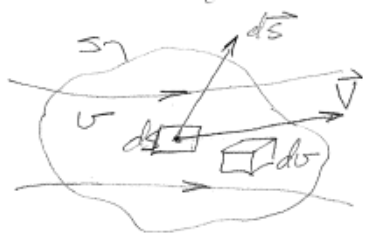
\includegraphics[width=0.4\linewidth]{Figures/pg28_1.PNG}
    \caption{Fluid flowing through a fixed control volume V}
    \label{fig:28_1}
\end{figure}

\paragraph*{} Apply the 1st Law to the fluid flowing through the control volume V, which is fixed in space. Let\\
$B_1$ = rate of heat added\\
$B_2$ = rate of work done\\
$B_3$ = rate of change of energy
\begin{equation*}
    B_1 + B_2 = B_3\qquad \text{1st Law}
\end{equation*}
Define $\dot{q}$ as the rate of heat addition for unit mass. Then for the control volume V:
\begin{equation*}
    \text{Rate of heat addition} = \volumeint\dot{q} \rho dV
\end{equation*}
Define $\dot{Q}_{visc}$ as the rate of heat addition due to viscosity. Then $B_1$ is the rate of heat addition.

\begin{figure}
    \centering
    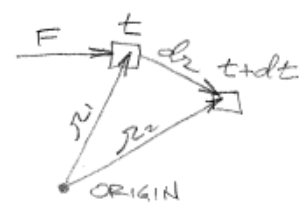
\includegraphics[width=0.3\linewidth]{Figures/pg29_1.PNG}
    \caption{Work done on object by forces}
    \label{fig:29_1}
\end{figure}

Consider the work done on an object by the force $\vec{F}$, where the position of the object is defined by the radius vector $\vec{r}$ with a fixed origin.\\
$Work = \vec{F} \bullet\vec{dr}$\\
Rate of work is
\begin{equation*}
    \vec{F}\bullet\frac{dr}{dt} \vec{F} \bullet\vec{V}
\end{equation*}
\paragraph{} On the surface S of the control volume, this pressure force is $-p\vec{ds}$
\begin{equation*}
    \text{Rate of work due to pressure} = -\oiint_S(p\vec{ds})\bullet\vec{V}
\end{equation*}

Similarly, recalling $\vec{f} =$ body force per unit mass, the rate of work due to body force is
\begin{equation*}
    \volumeint (\rho\vec{f} dv)\bullet \vec{V}
\end{equation*}
Define the rate of work due to shear as $\vec{\dot{w}}_{visc}$. Then $B_2$ (the rate of work done) is 
\begin{equation*}
    B_2 = -\iint_S p\vec{V}\bullet \vec{ds} + \volumeint \rho(\vec{f}\bullet\vec{V})dv + \dot{W}_{visc}
\end{equation*}
Internal energy is typically the energy due to random molecular motion for a stationary system. The energy within the control volume must also include the kinetic energy due to $\vec{V}$ Said kinetic energy/unit mass is $1/2V^2$. The mass flow across ds is $\rho \vec{V} \bullet \vec{ds}$.
\begin{equation*}
    \text{Rate of flow of energy} = \oiint_S (\rho \vec{V}\bullet \vec{ds})(e+\frac{V^2}{2})
\end{equation*}
\begin{equation*}
    \text{Time rate of change of energy in v} = \deldelt \volumeint \rho (e+\frac{V^2}{2})dv
\end{equation*}
Write $B_1 + B_2 = B_3$ (heat added + work done = rate of change of energy).
\begin{equation*}
    \volumeint \dot{q} \rho dv + \dot{Q}_{visc}
    -\iint_S p\vec{V}\bullet \vec{ds} + \volumeint \rho(\vec{f}\bullet\vec{V})dv + \dot{W}_{visc}
    = \deldelt \volumeint \rho(e+\frac{V^2}{2}) dv + \oiint_S (\rho \vec{V}\bullet \vec{ds})(e+\frac{V^2}{2})
\end{equation*}

Applying the divergence theorem to convert the surface integrals to volume integrals and setting the integrand = 0, we get Equation \ref{eq:EnergyBalance}.

\begin{equation}
    \deldelt \Big[ \rho(e+\frac{V^2}{2}) \Big] + \gradient \bullet \Big[ \rho(e+\frac{V^2}{2})\vec{V} \Big] =
    \rho \dot{q} - \gradient\bullet(\rho\vec{V}) + \rho (\vec{f}\bullet \vec{V}) + \dot{Q}_{visc} + \dot{W}_{visc}
    \label{eq:EnergyBalance}
\end{equation}
Where $\dot{Q}_{visc}$ and $\dot{W}_{visc}$ represent viscous terms to be defined explicitly later. Equation \ref{eq:EnergyBalance} is a PDE that defines the relationship of the flow field variables at any port in the control volume.

For the case of steady, inviscid, adiabatic flow with no body forces, the equations become Equation \ref{eq:SteadyInviscidEnergy}.
\begin{equation}
    \begin{array}{rcl}
    \oiint_S \rho (e+\frac{V^2}{2}) \vec{V} \bullet \vec{ds} &=& \oiint_S p\vec{V} \bullet \vec{ds} \\
    \gradient \bullet \Big[ \rho (e+\frac{V^2}{2})\vec{V} \Big] &=& -\gradient \dot (\rho \vec{V})
    \end{array}
    \label{eq:SteadyInviscidEnergy}
\end{equation}
For a calorically perfect gas: $e=C_v T$\\
For a perfect gas: $p=\rho RT$

\subsection{Substantial Derivative}
Consider a fluid element in a flow field from position 1 to 2. In general, flow properties are a function of both position and time, i.e. $\rho = \rho(x, y, z, t)$.\\
Using a Taylor series to expand this function about 1 (H.O.T. stands for Higher Order Terms):
\begin{equation*}
    \rho_2 = \rho_1 + \frac{\partial \rho}{\partial x}\Big)_1 (x_2=x_1)+ \frac{\partial\rho}{\partial y}\Big)_1 (y_2-y_1) + H.O.T.
\end{equation*}

\begin{equation*}
    \frac{\rho_2=\rho_1}{t_2-t_1} = \frac{\partial\rho}{\partial x}\Big)_1 \Big(\frac{x_2-x_1}{t_2-t_1}\Big) +
    \frac{\partial \rho}{\partial y}\Big)_1 \Big(\frac{y_2-y_1}{t_2-t_1}\Big) +
    \frac{\partial \rho}{\partial z}\Big)_1 \Big(\frac{z_2-z_1}{t_2-t_1}\Big)
\end{equation*}

Define the substantial derivative as Equation \ref{eq:SubstantialDerivative}.
\begin{equation*}
    \frac{Dp}{Dt}= \lim\limits_{t_2\rightarrow t_1} \frac{\rho_2-\rho_1}{t_2-t_1} \text{ and }
    \lim\limits_{t_2\rightarrow t_1} \frac{x_2-x_1}{t_2-t_1} = u_1
\end{equation*}
\begin{equation}
    \frac{D\rho}{Dt} = \frac{\partial \rho}{\partial t} + u \frac{\partial \rho}{\partial x} + v\frac{\partial \rho}{\partial y} + w\frac{\partial \rho}{\partial z}
    \label{eq:SubstantialDerivative}
\end{equation}
Physically, $D\rho /Dt$ is the rate of change of $\rho$ as the fluid element moves through space. $\partial \rho / \partial t$ is the rate of change of $\rho$ at a given point. For steady flow, $\partial \rho /\partial t = 0$ and $D\rho /Dt \neq 0$.

\paragraph*{} More generally
\begin{equation*}
    \frac{D}{Dt} = \deldelt + u\frac{\partial}{\partial x} + v \frac{\partial}{\partial y} + w\frac{\partial}{\partial z}
\end{equation*}
Recall the definition of the gradient:
\begin{equation}
    \gradient = \vec{i} \frac{\partial}{\partial x} + \vec{j} \frac{\partial}{\partial y} + \vec{k} \frac{\partial}{\partial z}
    \label{eq:Gradient}
\end{equation}
Thus
\begin{equation}
    \frac{D}{Dt} = \deldelt + (\vec{V} \bullet \gradient)
    \label{eq:SubstantialDerivative2}
\end{equation}
A useful vector identity is
\begin{equation*}
    \gradient \bullet (\rho \vec{V}) = \rho \gradient \bullet\vec{V} + \vec{V}\bullet\gradient\rho
\end{equation*}

Recall the continuity equation:
\begin{equation}
    \begin{array}{rcl}
    \frac{\partial \rho}{\partial t} + \gradient \bullet (\rho \vec{V}) &=& 0\\
    \text{Or } \frac{\partial \rho}{\partial t} + \vec{V} \bullet \gradient \rho + \rho \gradient \bullet \vec{V} &=& 0\\
    \frac{D\rho}{Dt} + \rho \gradient \bullet \vec{V} &=& 0
    \end{array}
    \label{eq:ContinuitySubstantialD}
\end{equation}
Equation \ref{eq:ContinuitySubstantialD} is the substantial derivative form of the continuity equation. Similarly the momentum equation becomes Equation \ref{eq:MomentumSubstantialD}.
\begin{equation}
    \rho \frac{Du}{Dt} = -\frac{\partial \rho}{\partial x} + \rho f_x + F_{x,visc} + \text{etc}
    \label{eq:MomentumSubstantialD}
\end{equation}
And the energy equation becomes Equation \ref{eq:EnergySubstantialD}.
\begin{equation}
    \rho \frac{D}{Dt} (e + \frac{V^2}{2}) = \rho \dot{q} - \gradient \bullet (\rho \vec{V}) + \rho (\vec{f} \bullet \vec{V}) + \dot{Q}_{visc} + \dot{W}_{visc}
    \label{eq:EnergySubstantialD}
\end{equation}

% PRAGMA MARK NEW SECTION, page 34
\section{Pathlines and Streamlines}
\begin{figure}
    \centering
    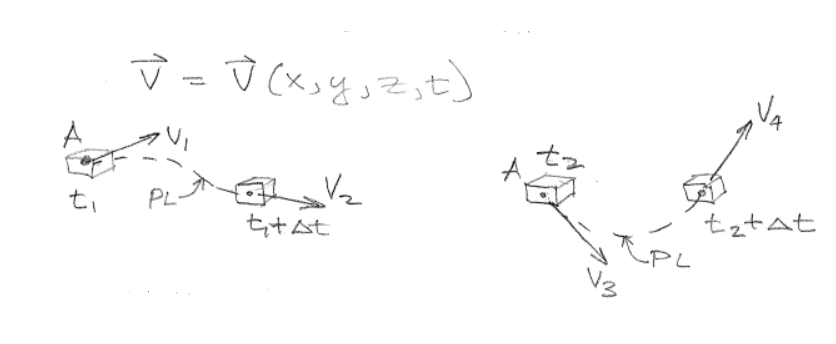
\includegraphics[width=0.9\linewidth]{Figures/pathline_streamline.PNG}
    \caption{Pathline and Streamline for a Fluid Element}
    \label{fig:PathlineStreamline}
\end{figure}

A \textbf{pathline} is the path a particular fluid element traces in space. At some time $t_1$, a fluid element passes through point A and traces the pathline shown in Figure \ref{fig:PathlineStreamline}. At some later time $t_2$, another fluid element passes through Point A and traces the pathline shown. If the flow is unsteady, the pathlines will be different.
 \paragraph*{} A streamline is a curve whose tangent is in the same direction as the velocity vector at that point.\\
 \textbf{Pathline $\rightarrow$ Time Exposure}\\
 \textbf{Streamline $\rightarrow$ Snapshot}\\
 For steady flows the streamlines and pathlines are the same.
 % "But what about the flow across the streamline?"
 
 \paragraph*{} Given a velocity field $\vec{V}(x, y, z)$, obtain the equation for the streamlines $f(x, y, z) = 0$. Let $\vec{ds}$ be an element of the streamline. For $\vec{ds}$ to be parallel to $\vec{V}$, it must be true that $\vec{ds} \times \vec{V} = 0$.
 
 \begin{equation*}
     \vec{ds} = dx\vec{i} + dy\vec{j} + dz\vec{k},\ \vec{V} = u\vec{i} + v\vec{j} + w\vec{k}
 \end{equation*}
 \begin{equation*}
    \vec{ds} \times \vec{V} =
    \begin{vmatrix}
    \vec{i} & \vec{j} & \vec{k} \\
    dx & dy & dz \\
    u & v & w\\
    \end{vmatrix} =
    \begin{matrix}\\\\ % weird notation is Liebeck's, sorry
    \vec{i} (wdy - vdz)\\
    + \vec{j}(udz - wdx)\\
    +\vec{k}(vdx - udy)\\
    \end{matrix} = 0
 \end{equation*}
 
 % after this point, emi got tired of writing \frac{\partial ...}{\partial ...}
 % this has been replaced with \partialfrac{...}{...}
 If a vector equals 0, all components are 0.
 \begin{equation*}
     \begin{matrix}
     wdy - vdz = 0\\
     udz - wdx = 0\\
     vdx - udy = 0\\
     \end{matrix}
 \end{equation*}
 In principle, if $u,\ v,\ w$ are known as functions of x, y, and z, these equations can be integrated to obtain the equation for the corresponding streamlines $f(x, y, z) = 0$. In 2D:
 \begin{figure}[ht]
     \centering
     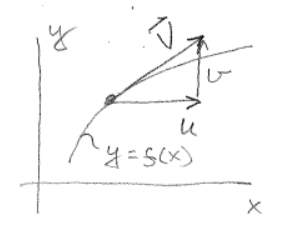
\includegraphics[width=0.3\linewidth]{Figures/2DStreamline.PNG}
     \caption{A Streamline in 2D Space}
     \label{fig:2DStreamline}
 \end{figure}
 The slope of the streamline is $dy/dx$ (Figure \ref{fig:2DStreamline}) and the slope of $\vec{V}$ is $v/u$. Since $dy/dx = v/u,\ vdx - udy = 0$.
 
 % Is anyone reading this source?
 \subsection{Vorticity, Strain}
 \begin{figure}[ht]
     \centering
     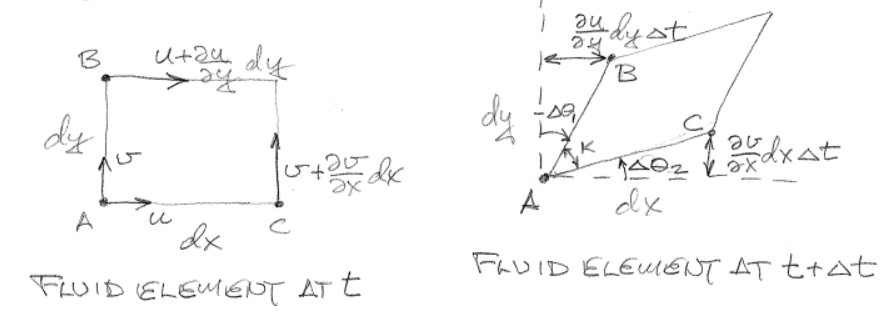
\includegraphics[width=0.9\linewidth]{Figures/VorticityStrain.PNG}
     \caption{Strain on a Fluid Element}
     \label{fig:VorticityStrain}
 \end{figure}
 In Figure \ref{fig:VorticityStrain}, consider the y-distance moved in $\Delta t$.
 At Point A, this distance is $v \Delta t$.\\
 At Point C, this distance is $(v + \partialfrac{v}{x}dx) \Delta t$.
 At Point C relative to Point A, $C-A = \partialfrac{v}{x}dx \Delta t$.\\
 The rotation of $\bar{AC}$ is
 \begin{equation*}
     \tan\Delta \theta_2 = \frac{\partialfrac{v}{x}dx \Delta t}{dx}= \partialfrac{v}{x}\Delta t
 \end{equation*}
 Or for small angles: $\Delta \theta_2 = \partialfrac{v}{x} \Delta t$.\\
 Similarly, for $\bar{AB},\
    \Delta \theta_1 = -\partialfrac{u}{y} \Delta t$.
\begin{equation*}
    \text{Taking the limit:} \lim\limits_{\Delta t\rightarrow 0} \frac{\Delta \theta_1}{\Delta t} =
    \frac{d\theta_1}{dt} - \partialfrac{u}{y},\quad \frac{d\theta_2}{dt} = \partialfrac{v}{x}
\end{equation*}
The angular velocity of the fluid element is the average of the angular velocities of $\bar{AB},\ \bar{AC}$. (Equation \ref{eq:2DAngularVelocity}.)
\begin{equation}
    \omega_2 = \frac{1}{2}\Big( \frac{d\theta_1}{dt} + \frac{d\theta_2}{dt} \Big) = \frac{1}{2}\Big(\partialfrac{v}{x} - \partialfrac{u}{y} \Big)
    \label{eq:2DAngularVelocity}
\end{equation}

Similar arguments apply in the yz and xz planes. The angular velocity in xyz-space is then Equation \ref{eq:3DAngularVelocity}.
\begin{equation}
    \omega = \frac{1}{2}\Bigg[ \Big( \partialfrac{w}{y} - \partialfrac{v}{z} \Big)\vec{i}
    + \Big( \partialfrac{u}{z} - \partialfrac{w}{x} \Big)\vec{j}
    + \Big( \partialfrac{v}{x} - \partialfrac{u}{y} \Big)\vec{k} \Bigg]
    \label{eq:3DAngularVelocity}
\end{equation}
For convenience, \textbf{vorticity} is defined as Equation \ref{eq:Vorticity}.
\begin{equation}
    \vec{\zeta} = 2\vec{\omega} % What's that snake-ass symbol? If you read the source you'll know.
    \label{eq:Vorticity}
\end{equation}

% It's 4:26 AM. (11.01.2018) Let's tell a story
% For the past two weeks, Liebeck has been warning us about the midterm.
% "I wrote the midterm", he likes to say, "and I gave it to Rayomand. And he made it harder."
% "But I talked him down," Liebeck says. "I don't want you to fail."
% He probably doesn't want bad rate my professor scores either.

Recalling the cross product of the operator $\gradient$ with $\vec{V}$:
\begin{equation}
    \gradient \times \vec{V} = \vec{\zeta}
    \label{eq:Vorticity2}
\end{equation}

The curl of velocity equals vorticity (Equation \ref{eq:Vorticity2}).\\
If $\gradient \times \vec{V} = 0$ everywhere, the flow is said to be \textbf{irrotational}. In the xy-plane, then:
\begin{equation}
    \partialfrac{v}{x} - \partialfrac{u}{y} = 0\ \text{(Irrotational Flow)}
    \label{eq:IrrotationalCondition}
\end{equation}

% 4:31 AM. Should I continue?
\subsection{Strain} % yes
The strain is defined as the change in the angle K of the fluid element. Strain is \textbf{positive} when K \textbf{decreases}.
\begin{equation*}
    \begin{array}{rcl}
    \Delta K &=& -\Delta \theta_2 = (-\Delta \theta_1)\\
    \text{Strain } = -\Delta K &=& \Delta \theta_2 - \Delta \theta_1 \\
    \end{array}
\end{equation*}

Recall $\Delta \theta_2 = \partialfrac{v}{x} \Delta t$ and $\Delta \theta_1 = \partialfrac{u}{y} \Delta t$. Define $\epsilon_{xy}$ as the rate of strain.
\begin{equation*}
    \epsilon_{xy} = -\frac{dK}{dt} = \frac{d\theta_2}{dt} - \frac{d\theta_1}{dt}
\end{equation*}
\begin{equation}
    \epsilon_{xy} = \partialfrac{v}{x} + \partialfrac{u}{y}
    \label{eq:Strain}
\end{equation}
\begin{equation*}
\begin{array}{rcl}
    \text{Similarly: } \epsilon_{yz} &=& \partialfrac{w}{y} + \partialfrac{v}{z}\\
    \epsilon_{zx} &=& \partialfrac{u}{z} + \partialfrac{w}{x}\\
    \end{array}
\end{equation*}

\begin{equation}
    \text{Write the matrix } \begin{bmatrix}
    \partialfrac{u}{x} & \partialfrac{u}{y} & \partialfrac{u}{z}\\
    \partialfrac{v}{x} & \partialfrac{v}{y} & \partialfrac{v}{z}\\
    \partialfrac{w}{x} & \partialfrac{w}{y} & \partialfrac{w}{z}\\
    \end{bmatrix}
    \label{eq:StrainMatrix}
\end{equation}
The diagonal of Equation \ref{eq:StrainMatrix} is $\gradient \bullet \vec{V}$ which is the dilatation of the element. The off-diagonal is the rotation and strain.
% 4:41 AM. Good night.

\subsection{Circulation}
\begin{figure}[ht]
    \centering
    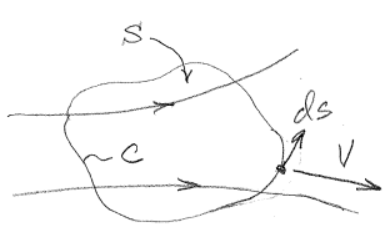
\includegraphics[width=0.3\linewidth]{Figures/circulation.PNG}
    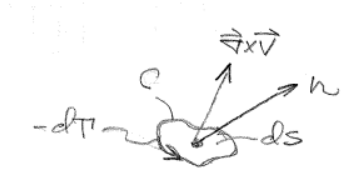
\includegraphics[width=0.3\linewidth]{Figures/circulation2.PNG}
    \caption{Circulation around a curve C in regular and differential form}
    \label{fig:Circulation}
\end{figure}

Define the circulation $\Gamma$ as Equation \ref{eq:Circulation}. This is minus due to clockwise $\Gamma$ being positive. 
\begin{equation}
    \Gamma = -\oint_C \vec{V} \bullet \vec{ds}
    \label{eq:Circulation}
\end{equation}
Consider S as any open surface bounded by C (Figure \ref{fig:Circulation}). From Stokes Theorem:
\begin{equation*}
    \Gamma = -\oint_C \vec{V} \bullet \vec{ds} = -\iint_S (\gradient \times \vec{V}) \bullet \vec{ds}
\end{equation*}
\begin{align*}
    \text{Letting C shrink to a point}\quad & d\Gamma = -(\gradient \times \vec{V}) \bullet \vec{ds} = -(\gradient \times \vec{V})\bullet \vec{n}ds\\
    \text{Divide by } ds \quad & \frac{d\Gamma}{ds} = -(\gradient \times \vec{V})\bullet \vec{n}\\
    \text{Recalling the definition of vorticity } \vec{\zeta} = \gradient \times \vec{V} \quad &
    \frac{d\Gamma}{ds} = -\vec{\zeta} \bullet \vec{n}\\
\end{align*}
The vorticity normal to ds is equivalent to the circulation per unit area (Figure \ref{fig:Circulation}).

\subsection{Stream Function}
Consider a 2D steady flow. Recall the differential equation for a streamline is $dy/dx = v/u$. If $u(x,y)$ and $v(x,y)$ are known, the differential equation can be integrated to obtain $f(x,y) = c$, an algebraic equation for the streamline. Call this function $\bar{\Psi}(x,y) = c$, the \textbf{stream function} (Figure \ref{fig:Streamfunction}).

\begin{figure}[ht]
    \centering
    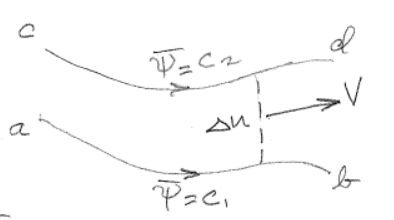
\includegraphics[width=0.4\linewidth]{Figures/streamfunction.PNG}
    \caption{Stream function and stream lines}
    \label{fig:Streamfunction}
\end{figure}

Different values of C will define different streamlines. Now define $\bar{\Psi}$ such that the difference $\Delta \bar{\Psi}$ between streamlines ab and cd is equal to the mass flow per unit depth.
\begin{equation*}
\Delta \bar{\Psi} = c_2 - c_1 = \text{Mass flow}
\end{equation*}
Continuity requires that this applies everywhere along the streamtube: $\Delta \bar{\Psi} = \rho V \Delta n$.
\begin{equation*}
    \rho V = \lim\limits_{\Delta n \rightarrow 0} \frac{\Delta \bar{\Psi}}{\Delta n} = \partialfrac{\bar{\Psi}}{u}
\end{equation*}

\begin{align*}
\text{Also from continuity:} \quad & \Delta \bar{\Psi} = \rho V \Delta n = \rho u \Delta y + \rho v(-\Delta x)\\
\text{Taking the limit:} & \quad d\bar{\Psi} = \rho u dy - \rho v dx\\
\text{Also for } \bar{\Psi} = \bar{\Psi} (x,y) & \quad d\bar{\Psi} = \partialfrac{\bar{\Psi}}{x}dx + \partialfrac{\bar{\Psi}}{y} dy \\
\text{Then:} & \quad \rho u = \partialfrac{\bar{\Psi}}{y},\quad \rho v = -\partialfrac{\bar{\Psi}}{x} \\
\end{align*}
For \textbf{incompressible flow}, define $\Psi = \bar{\Psi}/\rho$. Equation \ref{eq:StreamfunctionToVelocity} results. Given $\bar{\Psi}(x,y)$ or $\Psi(x,y)$, the velocities $u(x,y),\ v(x,y)$ can be obtained by differentiation.
\begin{equation}
    u = \partialfrac{\Psi}{y},\quad v = -\partialfrac{\Psi}{x}
    \label{eq:StreamfunctionToVelocity}
\end{equation}

\subsubsection{Stream Function in Polar Coordinates}
\begin{figure}[ht]
    \centering
    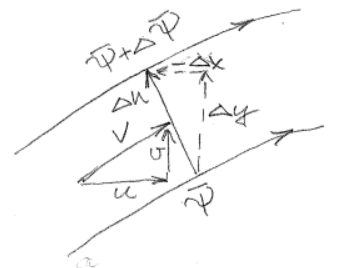
\includegraphics[width=0.4\linewidth]{Figures/polar_streamfunction.PNG}
    \caption{Stream function in Cartesian coordinates}
    \label{fig:PolarStreamfunction}
\end{figure}
\begin{align*}
    \text{Start with the definition} & \quad \Delta \bar{\Psi} = \rho V \Delta n \\
    \text{Then} & \quad \bar{\Psi} = (-\rho V_\theta)\Delta r + \rho V_r (r\Delta \theta)\\
    \text{Take the limit} & \quad d\Psi - =\rho V_\theta dr + \rho r V_r d\theta \\
    & \quad d\Psi = \partialfrac{\Psi}{r}dr + \partialfrac{\Psi}{\theta}d\theta\\
\end{align*}
\begin{equation}
\rho V_r = \frac{1}{r}\partialfrac{\bar{\Psi}}{\theta},\quad \rho V_\theta = -\partialfrac{\bar{\Psi}}{r}
    \label{eq:PolarStreamfunctionToVelocity}
\end{equation}

% PRAGMA MARK PAGE 43 VELOCITY POTENTIAL
\subsection{Velocity Potential}
Recall that if a flow is \textbf{irrotational}, Equation \ref{eq:Vorticity} is 0. $\vec{\zeta} = \gradient \times \vec{V} = 0$. Write the vector identity for a scalar function $\Phi(x,y)$ as $\gradient \times (\gradient \Phi) = 0$. If a flow is irrotational, there exists a scalar function $\Phi$ such that the velocity field is given by the gradient of $\Phi$.

\begin{align*}
    \text{Then} & \quad \vec{V} = \gradient \Phi = \partialfrac{\Phi}{x}\vec{i} + \partialfrac{\Phi}{y}\vec{j} + \partialfrac{\Phi}{z}\vec{k} \\
    \text{or} & \quad u = \partialfrac{\Phi}{x},\ v = \partialfrac{\Phi}{y},\ w = \partialfrac{\Phi}{z}\\
\end{align*}

\subsubsection{Relationship between Stream Function and Potential}
$\Phi$ = constant is an \textbf{equipotential line}.\\
A line everywhere tangent to $\gradient \Phi$ is a \textbf{gradient line}, and since $\gradient \Phi = \vec{V}$ this is also a streamline.\\
Gradient lines and equipotential lines are by definition \textbf{orthogonal}.
$\Psi$ = constant and $\Phi$ = constant are perpendicular.

\paragraph*{} For a 2D incompressible irrotational flow, $\Psi(x,y)$ = constant. Then, along a streamline:
\begin{equation*}
    d\Psi = \partialfrac{\Phi}{x}dx + \partialfrac{\Phi}{y}dy = 0
\end{equation*}
\begin{align*}
    \text{Also} & \quad d\Psi = -vdx + udy = 0\\
    \text{or} & \quad \frac{dy}{dx}\Big)_{\Phi = c} = \frac{v}{u}\\
\end{align*}
Similarly, $\Psi(x,y)$ = constant along an equipotential line, and:
\begin{equation*}
    d\Phi = \partialfrac{\Psi}{x}dx + \partialfrac{\Phi}{y}dy = 0
\end{equation*}
\begin{align*}
    \text{Also} & \quad d\Phi = udx + vdy\\
    \text{or} & \quad \frac{dy}{dx}\Big)_{\Phi = c} = -\frac{u}{v}\\
    \text{Then} & \quad \frac{dy}{dx}\Big)_{\Phi = c} = -\frac{1}{dy/dx\big)_{\Psi = c}}\\
\end{align*}

\begin{enumerate}
    \item u and v are obtained by differentiating $\Phi$ in the same direction as $\vec{V}$ and $\Psi$ in a direction normal to $\vec{V}$.
    \item $\Phi$ is defined for irrotational flow only. $\Psi$ does not require irrotational flow.
    \item $\Phi$ applies to 3D and 2D flow. $\Psi$ applies to 2D flow only.
\end{enumerate}

\subsubsection*{Velocity Potential in Polar Coordinates}
\begin{align*}
    \text{By definition} & \quad \vec{V} = \gradient \Phi \\
    \text{In polar coordinates} & \quad \gradient = \partialfrac{~}{r}\vec{e}_r + \frac{1}{r} \partialfrac{~}{\theta} \vec{e}_\theta \\
    \text{Then} & \quad \vec{V} = \partialfrac{\Phi}{r}\vec{e}_r + \frac{1}{r} \partialfrac{\Phi}{\theta}\vec{e}_\theta \\
\end{align*}
\begin{equation}
    V_r = \partialfrac{\Phi}{r},\ V_\theta = \frac{1}{r}\partialfrac{\Phi}{\theta}
    \label{eq:PolarPotentialToVelocity}
\end{equation}

% PRAGMA MARK NEW SECTION, page 46
\section{Bernoulli's Equation, Flow Measurement}
\subsection{Bernoulli's Equation}
Consider the case of a steady, incompressible, inviscid flow. Write the x-component of the momentual equation as:
\begin{align*}
    \text{Momentum} \quad & \rho \frac{Du}{Dt} = -\partialfrac{p}{x},\quad \partialfrac{u}{t} = 0\\
    \text{Expand and multiply by } dx \quad &
    u\partialfrac{u}{x} dx + v\partialfrac{u}{y}dx + w\partialfrac{u}{z}dx = -\frac{1}{\rho}\partialfrac{p}{x}dx\\
    \text{Consider 3D flow along a streamline} \quad & u dz - wdx \ 0\\
    & v dx - u dy = 0\\
    \text{Substituting} \quad &
    u\partialfrac{u}{x}dx + u\partialfrac{u}{y}dy + u\partialfrac{u}{z}dz = -\frac{1}{\rho}\partialfrac{p}{x}dx \\
    \text{Recall} \quad & du = \partialfrac{u}{x} dx + \partialfrac{u}{y}dy + \partialfrac{u}{z}dz \\
    & u du - -\frac{1}{\rho} \partialfrac{p}{x}dx \\
    \text{or similarly} \quad & \frac{1}{2}d(u^2) = -\frac{1}{\rho} \partialfrac{p}{x}dx \\
    & \frac{1}{2}d(v^2) = -\frac{1}{\rho} \partialfrac{p}{y}dy \\
    & \frac{1}{2}d(w^2) = -\frac{1}{\rho} \partialfrac{p}{z}dz \\
    \text{Also} \quad & dp = \partialfrac{p}{x}dx + \partialfrac{p}{y}dy + \partialfrac{p}{z}dz \\
    \text{Combine the 3 component equations} \quad & \frac{1}{2}d(V^2) = -\frac{1}{\rho}dp\\
\end{align*}
\begin{equation}
    dp = -\rho VdV
    \label{eq:EulerEq}
\end{equation}
Integrate Equation \ref{eq:EulerEq} between points 1 and 2 along a streamline:
\begin{equation*}
    \int_1^2 dp = -\rho \int_1^2 VdV,\ \rho\ \text{is constant}
\end{equation*}
\begin{equation}
    p_2 - p_1 = -\frac{1}{2}\rho (V_2^2 - V_1^2)
    \label{eq:BernoulliEq}
\end{equation}
Equation \ref{eq:BernoulliEq} shows that $p + 1/2\rho V^2$ is constant along a streamline. For the general case where the flow may be rotational, the constant will vary from streamline to streamline. For \textbf{irrotational flow}, $p + 1/2 \rho V^2$ everywhere. Thus, once the velocity field is known, the corresponding pressure field is known for a steady, incompressible, irrotational, inviscid flow.

\subsection{Incompressible Flow in a Duct}
\begin{figure}[ht]
    \centering
    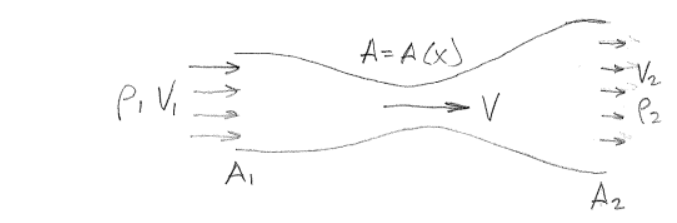
\includegraphics[width=0.5\linewidth]{Figures/flowInDuct.PNG}
    \caption{Incompressible flow in an axisymmetric duct}
    \label{fig:flowInDuct}
\end{figure}

Consider an axisymmetric duct (Figure \ref{fig:flowInDuct}) where the area change is gradual enough to assume one-dimensional flow. For steady flow, continuity requires
\begin{align*}
    \oiint_S \rho \vec{V} \bullet \vec{ds} &= 0\\
    \iint_{A_1} \rho \vec{V} \bullet \vec{ds} + \iint_{A+2} \rho \vec{V} \bullet \vec{ds} &= 0\\
    -\rho_1 A_1 V_1 + \rho_2 A_2 V_2 &= 0\ \text{ds positive outwards} \\
\end{align*}
\begin{equation*}
    \rho_1 A_1 V_1 \ \rho_2 A_2 V_2\ \text{or for incompressible flow}\ A_1V_1 \ A_2V_2
\end{equation*}

\subsubsection{Velocity in a Wind Tunnel}
\begin{figure}[ht]
    \centering
    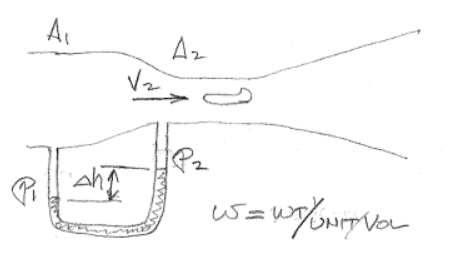
\includegraphics[width=0.5\linewidth]{Figures/flowInWindTunnel.PNG}
    \caption{Incompressible flow in a wind tunnel with a manometer}
    \label{fig:flowInWindTunnel}
\end{figure}
\begin{equation*}
    p_1 + \frac{1}{2}\rho V_1 ^2 = p_2 + \frac{1}{2}\rho V_2^2
\end{equation*}
\begin{equation*}
    V_2^2 = \frac{2}{\rho} (p_1-p_2) + \Big(\frac{A_2}{A_1}\Big)^2 V_2^2
    \quad \text{then} \quad
    V_2 = \sqrt{ \frac{2(p_1-p_2)}{\rho[1-(A_2/A_1)^2]} } =
    \sqrt{ \frac{2w\Delta h}{\rho[1-(A_2/A_1)^2]} }
\end{equation*}

\subsection{Measurement of Airspeed}
\begin{figure}[ht]
    \centering
    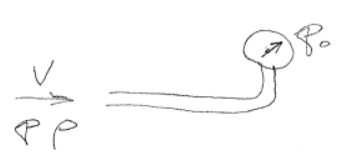
\includegraphics[width=0.3\linewidth]{Figures/pressureProbe.PNG}
    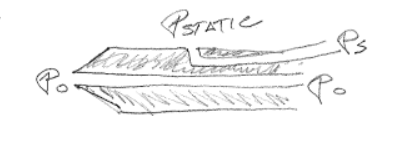
\includegraphics[width=0.3\linewidth]{Figures/pitotStaticProbe.PNG}
    \caption{Pressure probe (left) and pitot-static probe (right)}
    \label{fig:pressureProbes}
\end{figure}
Consider a pressure probe (Figure \ref{fig:pressureProbes}) pointing directly upstream. Then $p + 1/2 \rho V^2 = p_0$. $p_0$ is the stagnation pressure. For this probe:
\begin{equation*}
    V = \sqrt{ 2\frac{p_0-p}{\rho} }
\end{equation*}
The other probe in Figure \ref{fig:pressureProbes} is a \textbf{pitot probe}. Adding a static port and measuring the pressure difference $p_0-p$ gives the airspeed, assuming the density is known.
\begin{equation*}
    V\Big)_{IND} = \sqrt{ 2\frac{p_0-p}{\rho_{SL}} },\quad V\Big)_{TRUE} = \sqrt{2\frac{p_0-p}{\rho}}\quad  \text{and}\ V_{TRUE} = \sqrt{\frac{\rho_{SL}}{\rho}} V_{IND}
\end{equation*}
\subsubsection{Pressure Coefficient}
\begin{equation}
    C_P = \frac{p-p_\infty}{1/2\rho V_\infty^2} =
    \frac{1/2\rho (V_\infty^2 - V^2)}{1/2\rho V_\infty^2} =
    1-\Big(\frac{V}{V_\infty}\Big)^2
    \label{eq:PressureCoefficient}
\end{equation}

% PRAGMA MARK NEW SECTION page 50
\section{Incompressible, Inviscid Flow}
\subsection{Continuity Equation}
\begin{align*}
    \text{Recall the continuity equation} \quad & \partialfrac{\rho}{t} + \gradient \bullet\rho \vec{V} = 0\\
    \text{For steady, incompressible flow} \quad & \gradient \bullet \vec{V} = 0\\
\end{align*}
If in addition the flow is irrotational, there exists a velocity potential $\Phi$ where $\vec{V} = \gradient \Phi$. Then combine $\gradient \bullet (\gradient \Phi) = 0$ to obtain Equation \ref{eq:LaplaceGradientEq}: Laplace's Equation.
\begin{equation}
    \boxed{\nabla^2 \Phi = 0}
    \label{eq:LaplaceGradientEq}
\end{equation}

\begin{equation*}
    \nabla^2 \Phi = \frac{\partial^2 \Phi}{\partial x^2} + \frac{\partial^2 \Phi}{\partial y^2} + \frac{\partial^2 \Phi}{\partial z^2} = 0
\end{equation*}
Recall the stream function for \textbf{2D flow} (Equation \ref{eq:StreamfunctionToVelocity}).
\begin{equation*}
    u = \partialfrac{\Psi}{y},\quad v = -\partialfrac{\Psi}{x}
\end{equation*}
\begin{align*}
    \text{The 2D continuity equation is} \quad &
    \gradient \bullet \vec{V} = \partialfrac{u}{x} + \partialfrac{v}{y} = 0\\
    \text{In terms of } \Psi\ \text{this becomes} \quad & \frac{\partial^2 \Psi}{\partial x \partial y} - \frac{\partial^2 \Psi}{\partial y \partial x} = 0\ \text{(trivial)}\\
\end{align*}

Recall Equation \ref{eq:IrrotationalCondition}: $\partialfrac{v}{x} - \partialfrac{u}{y} = 0$ (condition for irrotational flow). In terms of $\Psi$ this becomes:
\begin{equation*}
    \frac{\partial^2 \Psi}{\partial x^2} + \frac{\partial^2 \Psi}{\partial y^2} = 0\quad \text{Laplace's Equation}
\end{equation*}

\begin{enumerate}
    \item Any irrotational, incompressible flow has a velocity potential that satisfies Laplace's Equation. If the flow is 2D, it has a stream function that also satisfies Laplace's Equation.
    \item Conversely, any solution to Laplace's Equation represents $\Phi$ or $\Psi$ for a flow.
    \item Since Laplace's Equation is linear, separate solutions may be summed to obtain a combined solution $\Phi = \Phi_1 + \Phi_2 + ...$
\end{enumerate}

\subsection{Boundary Conditions}
\begin{align*}
    \text{At infinity} \quad & u = \partialfrac{\Phi}{x} = \partialfrac{\Psi}{y} = V_\infty \\
    & v = \partialfrac{\Phi}{y} = -\partialfrac{\Psi}{x} = 0\\
    \text{At the body} \quad & \vec{V}\bullet \vec{n} = \gradient \Psi \bullet \vec{n} = 0\\
    & \partialfrac{\Phi}{n} = 0\\
    & \Psi_{surface} = \text{const} \\
    & \partialfrac{\Psi}{s} = 0\\
    \text{For 2D flows} \quad & \frac{dy_{body}}{dx} = \frac{v}{u}\Big)_{surface} \\
\end{align*}
Note: for viscous flows, the velocity is zero at the wall.

\subsection{Uniform Flow}
Consider uniform flow in the x-direction: $\gradient \bullet \vec{V} = 0$ for incompressible flow, and $\gradient \times \vec{V} = 0$ for irrotational flow. \textbf{This is physically possible!} (Equation \ref{eq:UniformFlow}.)
\begin{equation}
    u = \partialfrac{\Phi}{x} = V_\infty \quad v = \partialfrac{\Phi}{y} = 0
    \label{eq:UniformFlow}
\end{equation}

\begin{align*}
    \text{Integrating with respect to x} \quad &
    \Phi = V_\infty x + f(y)\\
    \text{Integrating with respect to y} \quad & \Phi = const + q(x)\\
\end{align*}
Since $\Phi(x,y)$ is the same function, $q(x) = V_\infty x + const$. $\Phi$ is always differentiated to obtain velocity, so the constant can be omitted.
\begin{equation*}
    \boxed{\Phi = v_\infty x} \quad \text{Uniform flow velocity potential}
\end{equation*}

Similarly, from $u = \partialfrac{\Psi}{y} = V_\infty$ and $v = -\partialfrac{\Psi}{x} = 0$, the stream function becomes
\begin{equation*}
    \boxed{\Psi = v_\infty y} \quad \text{Uniform flow stream function}
\end{equation*}

\subsubsection{Uniform Flow in Polar Coordinates}
\begin{figure}[ht]
    \centering
    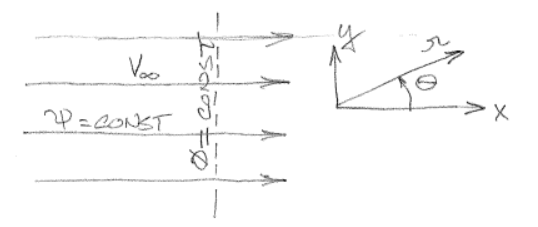
\includegraphics[width=0.5\linewidth]{Figures/UniformFlow.PNG}
    \caption{Uniform flow in polar coordinates}
    \label{fig:UniformFlow}
\end{figure}
\begin{align*}
    \text{In polar coordinates} \quad & \Phi = V_\infty r \cos(\theta) \\
    & \Psi = V_\infty r \sin(\theta) \\
    V_r = \partialfrac{\Phi}{r} = V_\infty \cos(\theta),\quad & V_\theta = \frac{1}{r} \partialfrac{\Phi}{\theta} = -V_\infty \sin(\theta) \\
    V_r = \frac{1}{r} \partialfrac{\Psi}{\theta} = V_\infty \cos(\theta), \quad & V_\theta = -\partialfrac{\Psi}{r} = -V_\infty \sin(\theta) \\
\end{align*}

\subsection{Source (Sink) Flow}
\begin{figure}[ht]
    \centering
    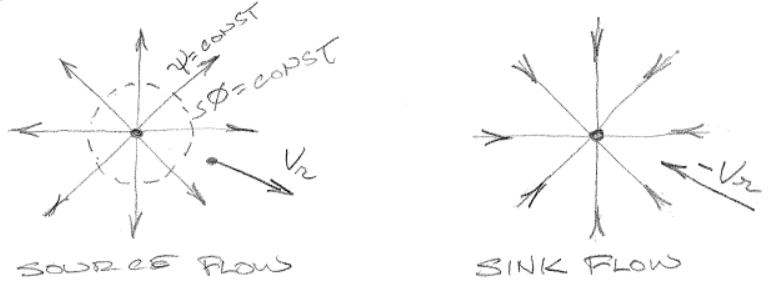
\includegraphics[width=0.8\linewidth]{Figures/sourceSinkFlow.PNG}
    \caption{Source and Sink Flow}
    \label{fig:SourceSinkFlow}
\end{figure}
\begin{align*}
\text{Source or sink flow is defined by} \quad & V_r = c/r,\quad V_\theta = 0\\
\text{Check continuity} & \quad \gradient \bullet \vec{V} = 0\\
\gradient \bullet \vec{V} &= \frac{1}{r} \partialfrac{}{r}(rV_r) + \frac{1}{r} \partialfrac{V_\theta}{\theta}\\
\gradient \bullet \vec{V} & =\frac{1}{r} \partialfrac{}{r} (r \times \frac{c}{r}) = 0\\
\end{align*}
Similarly, $\gradient \times \vec{V} = 0$ so the flow is irrotational.

\begin{figure}[ht]
    \centering
    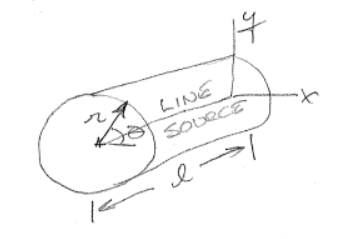
\includegraphics[width=0.4\linewidth]{Figures/lineSourceFlow.PNG}
    \caption{Line Source Flow}
    \label{fig:LineSourceFlow}
\end{figure}
Consider a line source (Figure \ref{fig:LineSourceFlow}) of length $l$ normal to the xy-plane. At a radius $r$, define:
\begin{align*}
    \vec{ds} &= l\vec{r} d\theta \\
    d\dot{m} &= \rho \vec{V} \bullet \vec{ds} = \rho V_r lr d\theta \\
    \dot{m} &= \int_0^{2\pi} \rho V_r lr d\theta = 2\pi \rho lr V_r \quad \text{mass/unit time} \\
\end{align*}

Define $\dot{v} = \dot{m}/\rho$ as the volume flow / unit time. Then $\dot{v} = 2\pi lr V_r$.\\
Next, define $\Lambda = \dot{v}/l$ as the volume flow rate / unit length. Then $\Lambda = 2\pi rV_r$.
\begin{equation*}
    V_r = \frac{\Lambda}{d\pi r} \quad \Lambda = \text{Source strength, negative for sink}
\end{equation*}

\subsubsection{Velocity Potential for a Source}
\begin{align*}
    V_r &= \partialfrac{\Phi}{r} = \frac{\Lambda}{2\pi r} \\
    V_\theta &= \frac{1}{r} \partialfrac{\Phi}{\theta} = 0 \\
    \text{Integrating } \Phi &= \frac{\Lambda}{2\pi}\log(r) + f(\theta) \\
    \Phi &= const + f(r) \\
\end{align*}
\begin{equation*}
    \boxed{\Phi = \frac{\Lambda}{2\pi}\log(r)} \quad \text{Velocity potential for a source}
\end{equation*}

\subsubsection{Stream Function for a Source}
\begin{align*}
    V_r = \frac{1}{r} \partialfrac{\Psi}{\theta} = \frac{\Lambda}{2pi r}, \quad & V_\theta = -\partialfrac{\Psi}{r} = 0 \\
    \text{Integrating } \Psi &= \frac{\Lambda}{2\pi}\theta + f(r)\\
\end{align*}
Notice that for $\Psi = const$ (streamline), $\theta=const$ which is a line from the origin.
\begin{equation*}
    \boxed{\Psi = \frac{\Lambda}{2\pi}\theta} \quad \text{Stream function for a source}
\end{equation*}

% PRAGMA MARK NEW SUBSECTION source & sink page 57
\subsection{Uniform Flow + Source and Sink}
\begin{figure}[ht]
    \centering
    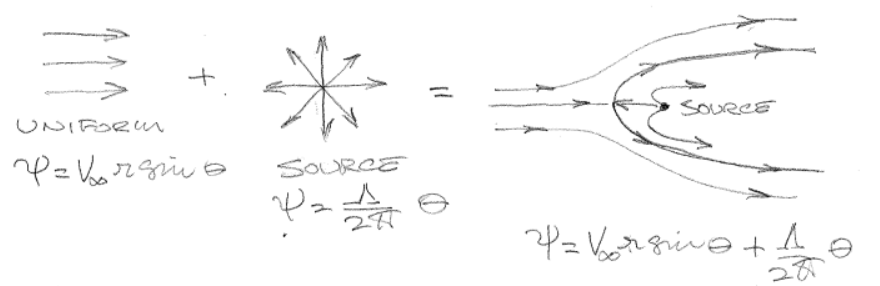
\includegraphics[width=0.8\linewidth]{Figures/uniformPlusSourceFlow.PNG}
    \caption{Uniform Flow + Source}
    \label{fig:UniformPlusSourceFlow}
\end{figure}
In Figure \ref{fig:UniformPlusSourceFlow} 2 flows are superimposed. Both satisfy Laplace's equation, so the combination satisfies Laplace's equation. The stagnation point is defined by:
\begin{align*}
    V_r &=\frac{1}{r} \partialfrac{\Psi}{\theta} = V_\infty \cos(\theta) + \frac{\Lambda}{2\pi r} = 0\\
    V_\theta &= -\partialfrac{\Psi}{r} = -V_\infty \sin(\theta) = 0\\
    r &= \frac{\Lambda}{2\pi V_\infty},\quad \theta = \pi\\
\end{align*}

Note the effect of $V_\infty$ and $\Lambda$:\\
Increasing $\Lambda$ moves the stagnation point forward.\\
Increasing $V_\infty$ moves the stagnation point aft.

\begin{equation*}
\text{Substitute } \frac{\Lambda}{2\pi V_\infty},\ \pi\ \text{into } \Psi \quad
\Psi = V_\infty \frac{\Lambda}{2\pi V_\infty}\sin(\pi) + \frac{\Lambda}{2\pi}\pi = \frac{\Lambda}{2} =\ \text{Body streamline}
\end{equation*}
Because it contains the stagnation point, this streamline divides the source flow from the freestream.

\subsubsection{Rankine Oval}
\begin{figure}[ht]
    \centering
    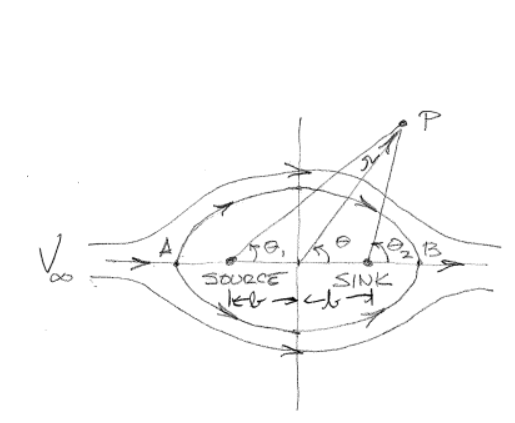
\includegraphics[width=0.5\linewidth]{Figures/rankineOval.PNG}
    \caption{Rankine Oval formed by uniform flow, source, and sink}
    \label{fig:RankineOval}
\end{figure}
Consider a source sink pair equidistant (distance b) from the origin in a uniform flow (Figure \ref{fig:RankineOval}).
\begin{align*}
    \Psi &= V_\infty r\sin(\theta) + \frac{\Lambda}{2\pi}\theta_1 - \frac{\Lambda}{2\pi}\theta_2\\
    \text{or } \Psi &= V_\infty r\sin(\theta) + \frac{\Lambda}{2\pi} (\theta_1-\theta_2)
\end{align*}

Note: $\theta_1,\ \theta_2$ are functions of $(r, \theta)$ and b. To solve for the stagnation points A and B, first note that by symmetry they must lie on $\theta = 0,\ \pi$ and $V_\theta = 0$.

\begin{align*}
    \text{At point A: Freestream} &= +V_\infty \\
    V_{SOURCE} &= -V_r = -\frac{\Lambda}{2\pi(r-b)}\\
    V_{SINK} &= -V_r = -\frac{-\Lambda}{2\pi(\pi + b)}\\
    V_a &= V_\infty + \frac{\Lambda}{2\pi} \Big( \frac{1}{\pi + b} - \frac{1}{\pi - b}\Big) = 0\ \text{for stagnation} \\
    V_a &= V_\infty + \frac{\Lambda}{2\pi} \Big[ \frac{(r-b)-(+b)}{(\pi-b)(\pi+b)} \Big] = V_\infty + \frac{\Lambda}{2\pi} \frac{-2b}{\pi^2 - b^2} = 0\\
    r &= \sqrt{ \frac{\Lambda b}{\pi V_\infty} + b^2 }
\end{align*}

The equation for a streamline is again:
\begin{equation*}
    \Phi = V_\infty r\sin(\theta) + \frac{\Lambda}{2\pi}(\theta_1-\theta_2) = const
\end{equation*}
The streamline for the body contains the stagnation point A where $\theta = \theta_1 = \theta_2 = \pi$ and point B where $\theta = \theta_1 = \theta_2 = 0$. Substituting in the stream function gives:
\begin{equation*}
    V_\infty r \sin(\theta) + \frac{\Lambda}{2\pi}(\theta_1-\theta_2) = 0
\end{equation*}
This can be shown to be the equation of an oval called the \textbf{Rankine oval}.

% "You'll have me again next quarter...if you survive this one." ~Liebeck

\subsection{Doublet Flow}
\begin{figure}[ht]
    \centering
    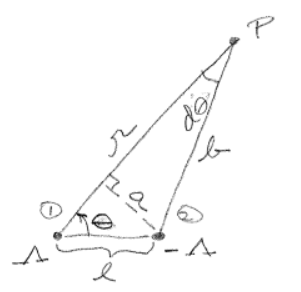
\includegraphics[width=0.3\linewidth]{Figures/doubletFlow.PNG}
    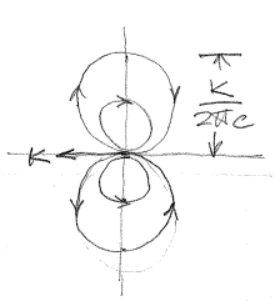
\includegraphics[width=0.3\linewidth]{Figures/doubletFlow2.PNG}
    \caption{Doublet flow at a point P and on the xy-plane}
    \label{fig:DoubletFlow}
\end{figure}
Consider a source sink pair at a distance $l$ from each other (Figure \ref{fig:DoubletFlow}).
\begin{equation*}
    \Psi = \frac{\Lambda}{2\pi}(\theta_1 - \theta_2) = -\frac{\Lambda}{2\pi}\Delta \theta \quad \Delta \theta = \theta_2-\theta_1
\end{equation*}
Let $l\rightarrow 0$ while $l\Lambda = K$ remains constant.
\begin{equation*}
    \Psi = \lim\limits_{l\rightarrow 0,\ K \rightarrow l\Lambda} \Big(-\frac{\Lambda}{2\pi} d\theta \Big) \quad \Lambda \rightarrow \infty\ \text{as}\ l \rightarrow 0
\end{equation*}
For small $\Delta \theta \rightarrow d\theta \rightarrow 0$:
\begin{align*}
    a &= l\sin\theta, \quad
    b = r - l\cos\theta, \quad
    d\theta = a/b = \frac{l\sin\theta}{r-l\cos\theta}\\
    \Psi &= \lim\limits_{l\rightarrow 0,\ K = \Lambda l} \Big( -\frac{\Lambda l \sin\theta}{2\pi (r-l\cos\theta)} \Big) =
    \lim\limits_{l\rightarrow 0,\ K = \Lambda l} \Big( -\frac{K\sin\theta}{2\pi(r-\cos\theta)} \Big) \\
    \Psi &= -\frac{K\sin\theta}{2\pi r}\ K =\ \text{doublet strength}
\end{align*}

To obtain the velocity potential, recall
\begin{equation*}
    V_r = \partialfrac{\Phi}{r} = \frac{1}{r}\partialfrac{\Psi}{\theta} = -\frac{K\cos(\theta)}{2\pi r^2}
\end{equation*}
\begin{align*}
    \text{Integrating with respect to } r\quad & \Phi = -\frac{K}{2\pi}\big(-\frac{1}{r}\big)\\
    \text{or}\quad & \Phi = \frac{K}{2\pi}\cos(\theta)\\
    \text{For the streamlines}\quad & \Psi = -\frac{K\sin(\theta)}{2\pi r} = const = c\\
    \text{or}\quad & r =-\frac{K}{2\pi c}\sin(\theta)
\end{align*}
The family of circles corresponds to the streamlines in Figure \ref{fig:DoubletFlow}.

% PRAGMA MARK page 62, halfway point, flow over circular cylinder
\subsection{Flow over a Circular Cylinder}
\begin{figure}[ht]
    \centering
    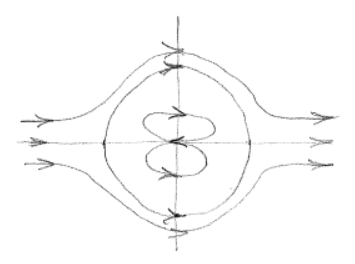
\includegraphics[width=0.3\linewidth]{Figures/flowCircularCylinder.PNG}
    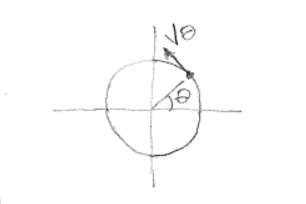
\includegraphics[width=0.3\linewidth]{Figures/flowCircularCylinder2.PNG}
    \caption{Flow over a circular cylinder constructed using a uniform flow and doublet}
    \label{fig:FlowCircularCylinder}
\end{figure}

Consider the combination of a uniform flow and doublet (Figure \ref{fig:FlowCircularCylinder}).
\begin{align*}
    \Psi &= V_\infty r\sin(\theta) - \frac{K\sin(\theta)}{2\pi r}\\
    \text{Let } R^2 &= \frac{K}{2\pi V_\infty}\\
    \Psi &= V_\infty r\sin(\theta)\big( 1-\frac{R^2}{r^2} \big)\\
    V_r &= \frac{1}{r} \partialfrac{\Psi}{\theta} = \Big(1=\frac{R^2}{r^2}\Big)  V_\infty \cos(\theta)\\
    V_\theta &= -\partialfrac{\Psi}{r} = -\Big[ \big( V_\infty r\sin(\theta) \big)\frac{2R^2}{r^3} + \big( 1-\frac{R^2}{r^2} \big) V_\infty \sin(\theta) \Big] = -\Big( 1+\frac{R^2}{r^2} \Big) V_\infty \sin(\theta)
\end{align*}

Solve for the stagnation point by setting $V_r = V_\theta = 0$.
\begin{equation*}
    \Big( 1-\frac{R^2}{r^2} \Big) V_\infty \cos\theta = 0, \quad \Big( 1 + \frac{R^2}{r^2} \Big) V_\infty \sin\theta = 0
\end{equation*}

Stagnation occurs at 2 points: $(R,0),\ (R,\pi)$. Also, the corresponding streamline containing the stagnation points is:
\begin{equation*}
    \Psi = V_\infty r \sin(\theta)\big( 1-\frac{R^2}{r^2}\big) = 0
\end{equation*}
For $r=R$, this is satisfied for all values of $\theta$. Thus $\Psi = 0$ is a circle of radius:
\begin{equation*}
    R = \sqrt{\frac{\kappa}{2\pi V_\infty}}
\end{equation*}
on the cylinder $r \ R$. $V_\theta = -2V_\infty \sin(\theta),\ V_r \ 0$.\\

Recalling Equation \ref{eq:PressureCoefficient} we can write:
\begin{equation*}
    C_p = 1-\Big(\frac{V}{V_\infty}\Big)^2 = 1-4\sin^2\theta
\end{equation*}
It is observed that the flow, and hence the pressure distribution, is \textbf{symmetric top and bottom and face and aft}. Thus there is no lift force and \textbf{no drag force}. This is called \textbf{D'Alembert's Paradox}. The pressure is symmetrically distributed (Figure \ref{fig:CpCircularCylinder}).
\paragraph*{} This holds for all potential flow solutions without circulation, since there are no viscous forces and no separation.

\begin{figure}[ht]
    \centering
    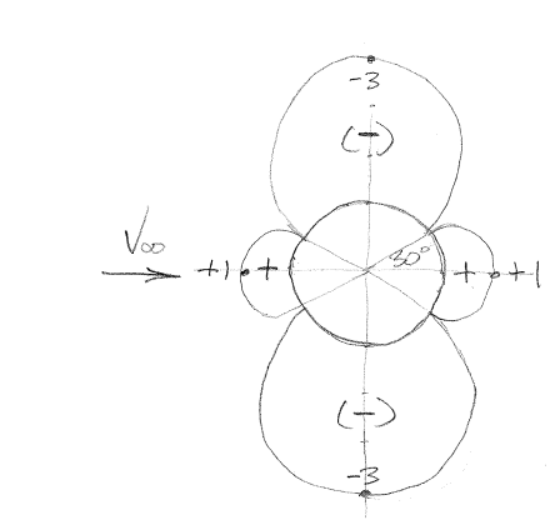
\includegraphics[width=0.3\linewidth]{Figures/CpOnCylinder.PNG}
    \caption{Polar plot of pressure coefficient $C_p$ on a circular cylinder}
    \label{fig:CpCircularCylinder}
\end{figure}

% LPT: get a loud keyboard. The noise will keep you awake working late.

\subsection{Vortex Flow}
\begin{figure}[ht]
    \centering
    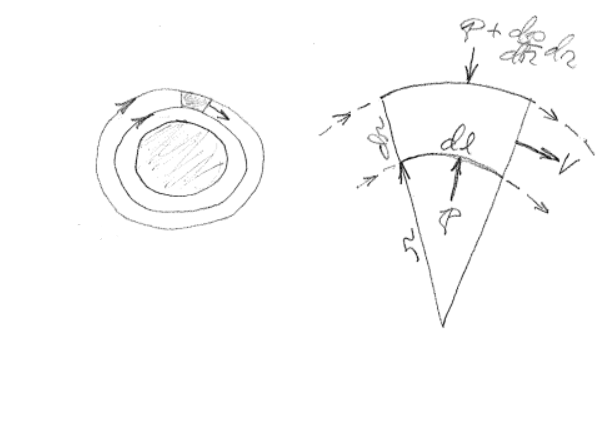
\includegraphics[width=0.3\linewidth]{Figures/vortexFlow.PNG}
    \caption{Vortex flow streamlines and differential element}
    \label{fig:VortexFlow}
\end{figure}

Consider the flow of a fluid in concentric circles. For equilibrium, the centrifugal force must be balanced by the pressures on the surface of the element (Figure \ref{fig:VortexFlow}).
\paragraph*{} Assuming unit thickness, the volume of the element is $dldr$, and the centrifugal force is $(\rho dldr) V^2/r$. The net pressure force acting toward the center is:
\begin{equation*}
    \big( p+ \frac{dp}{dr}dr \big) dl - pdl = \frac{dp}{dr}drdl
\end{equation*}
\begin{align*}
    \text{Isolating the forces} \quad &
    \frac{dp}{dr} = =\rho \frac{V^2}{r}\\
    \text{Euler's Equation} \quad &
    dp = -\rho VdV\\
    \text{Then} \quad & -\rho V \frac{dV}{dr} = \rho \frac{V^2}{r}\\
    \text{or} \quad & \frac{dV}{V} = -\frac{dr}{r}\\
    \text{Integrating} \quad & \log(V) = -\log(r) + const\\
    \text{then} \quad & \log(Vr) = const
\end{align*}

\begin{equation}
    \text{Vortex flow} \quad V = \frac{\text{const}}{r} \quad V_r = 0 \quad V_\theta = \frac{c}{r}
     \label{eq:VortexFlow}
\end{equation}
 
 Calculate the circulation $\Gamma$ around a circular streamline of radius r:
 \begin{equation*}
     \Gamma = -\oint_C \vec{V} \bullet ds = -V_\theta 2\pi r = \frac{c}{r} 2\pi r = 2\pi c \quad \text{then} \quad v = -\frac{\Gamma}{2\pi}
 \end{equation*}
 \begin{equation*}
     \boxed{V_\theta= -\frac{\Gamma}{2\pi r}} \quad \text{positive } \Gamma\ \text{is clockwise}
 \end{equation*}
 
 To check on irrotationality, recall Equation \ref{eq:Circulation} (definition of circulation).
 \begin{equation*}
     \Gamma = -\iint_S (\gradient \times \vec{V}) \bullet \vec{ds} = -2\pi c
 \end{equation*}
 Fo a 2D flow, $\gradient \times \vec{V}$ and $\vec{ds}$ are both normal to the plane of the flow; thus
 \begin{equation*}
     2\pi c = \iint_S \big| \gradient \times \vec{V} \big| ds
 \end{equation*}
 Next, since $\Gamma$ is invariant with $r$, let $r \rightarrow 0$ while $\Gamma = -2\pi c$.
 \begin{align*}
     \text{Then} \quad & \iint \big| \gradient \times \vec{V} \big| ds \rightarrow \big| \gradient \times \vec{V} \big| ds\\
     \text{or} \quad & 2\pi c = \big| \gradient \times \vec{V} \big| ds\\
     \text{then} \quad & \big| \gradient \times \vec{V} \big| \rightarrow \infty \quad \text{as } r \rightarrow 0
 \end{align*}
 
 Vortex flow is irrotational everywhere except at $r=0$ where the vorticity is infinite.
 For the velocity potential:
 \begin{align*}
     \frac{1}{r} \partialfrac{\Phi}{\theta} &= V_\theta = -\frac{\Gamma}{2\pi r}, \quad \partialfrac{\Phi}{r} = V_r = 0\\
     \partialfrac{\Phi}{\theta} &= -\frac{\Gamma}{2\pi} \\
     \text{Integrating} \quad \Phi &=-\frac{\Gamma}{2\pi}\theta + f(r)\\
     \Phi & = f(\theta) \\
     \text{then} \quad \Phi &= -\frac{\Gamma}{2\pi}\theta 
 \end{align*}
 For the stream function:
 \begin{align*}
     \frac{1}{r} \partialfrac{\Psi}{\theta} &=V_r = 0,\quad -\partialfrac{\Psi}{\theta} = V_\theta = -\frac{\Gamma}{2\pi r}\\
     \text{Integrating} \quad \Psi &= f(r) \\
     \Psi & = \frac{\Gamma}{2\pi}\log(r) + f(\theta)\\
     \text{then} \quad \Psi &= \frac{\Gamma}{2\pi}\log(r)
 \end{align*}
 
 \subsection{Circular Cylinder with Lift}
 The stream function for a vortex can be written with an arbitrary constant of integration:
 \begin{align*}
     \Psi &=\frac{\Gamma}{2\pi} \log(r) + const\\
     \text{Therefore, set} \quad const &= -\frac{\Gamma}{2\pi}\log (R)\\
     \text{and } \Psi\ \text{becomes} \quad \Psi &= \frac{\Gamma}{2\pi} \log\big(\frac{r}{R}\big)
 \end{align*}
 Adding this to $\Psi$ for the flow about a cylinder, we get the following equation where again $\Psi = 0$ for $r = R$.
 \begin{equation*}
     \Psi = V_\infty r \sin\theta \big(1-\frac{R^2}{r^2}\big) + \frac{\Gamma}{2\pi}\log\big(\frac{r}{R}\big)
 \end{equation*}
 
 % PRAGMA MARK subsection stagnation points page 68
 \subsection{Stagnation Points}
 \begin{figure}[ht]
     \centering
     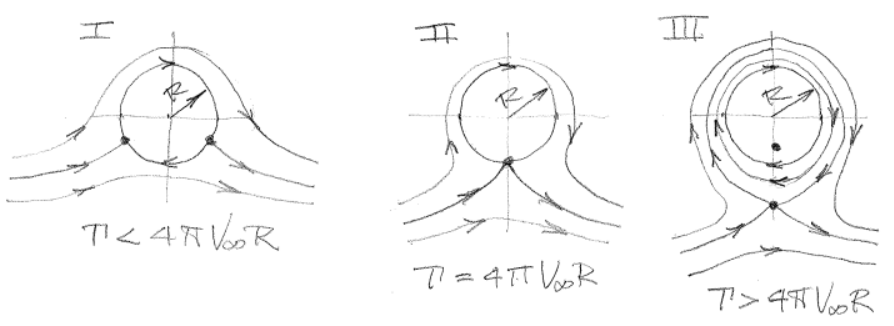
\includegraphics[width=0.8\linewidth]{Figures/stagnationPoints.PNG}
     \caption{Stagnation points on a cylinder for varying values of $\Gamma$}
     \label{fig:StagnationPoints}
 \end{figure}
 Set the velocity equal to 0 (condition for a stagnation point).
 \begin{align*}
     V_r &= \frac{1}{r} \partialfrac{\Psi}{\theta} = \Big( 1-\frac{R^2}{r^2} \Big)V_\infty \cos\theta = 0\\
     V_\theta &= -\partialfrac{\Psi}{r} = -\Big( 1+\frac{R^2}{r^2}\Big) V_\infty \sin\theta - \frac{\Gamma}{2\pi r} = 0
 \end{align*}
 On the cylinder, $r=R$.
 \begin{equation*}
     \theta \big|_{STAG} = \sin^{-1}\big( -\frac{\Gamma}{4\pi V_\infty R} \big)
 \end{equation*}
 Since $\Gamma > 0$, therefore $\theta > \pi$. There are three cases (Figure \ref{fig:StagnationPoints}):
 \begin{enumerate}
     \item $\Gamma < 4\pi V_\infty R$: 2 stagnation points symmetric about $3\pi/2$
     \item $\Gamma = 4\pi V_\infty R$: 1 stagnation point at $3\pi/2$
     \item $\Gamma > 4\pi V_\infty R$: Return to equation for $V_r = 0$ also satisfied by $\theta = \pm \pi/2$. Then $$\theta = \mp \Big( 1+\frac{R^2}{r^2} \Big)V_\infty - \frac{\Gamma}{2\pi r} = 0$$
    Solve for R
    \begin{equation*}
        r = \frac{\Gamma}{4\pi V_\infty} \pm \sqrt{ \Big( \frac{\Gamma}{4\pi V_\infty} \Big)^2 - R^2 }
    \end{equation*}
    There are 2 stagnation points, one inside and one outside. (There exists a theoretical flow inside the cylinder, just as with the simple doublet.) The flow outside $r=R$ is the only one of interest, and it has the single \textbf{off-body} stagnation point.
 \end{enumerate}
 
 % sqlserver is the best Overleaf editor theme
 % Don't @ me
 
 \subsection{Lift and Drag}
 The velocity on the surface of the cylinder is $V=V_\theta = -2V_\infty \sin(\theta) = \Gamma/(2\pi r)$. Then
 \begin{equation*}
     C_p = 1-\big( \frac{V}{V_\infty} \big)^2 = 1-\Big[ 4\sin^2(\theta) + \frac{2\Gamma \sin(\theta)}{\pi RV_\infty} + \big(\frac{\Gamma}{2\pi RV_\infty}\Big)^2 \Big]
 \end{equation*}

 Recall the equation for $Cd$:
 \begin{equation*}
     C_d = \frac{1}{c} \int_{LE}^{TE} C_{p_u} dy - \int_{LE}^{TE}C_{P_l}dy
 \end{equation*}

 Transform to polar coordinates: $y = R\sin(\theta),\ dy = R\cos(\theta),\ c=2R$
 \begin{gather*}
 C_d = \frac{1}{2} \int_\pi ^0 C_{p_u} \cos(\theta) d\theta - \frac{1}{2}\int_\pi^{2\pi}C_{p_l}\cos(\theta)d\theta\\
 \text{Note:}\quad LE \rightarrow TE\big)_u \Longrightarrow \pi \rightarrow 0,\quad LE \rightarrow TE\big)_l\Longrightarrow \pi \rightarrow 2\pi\\
 C_d = -\frac{1}{2}\int_0^{2\pi} C_D \cos(\theta) d\theta\\
 \text{Substitute} \quad C_p(\theta)\ \text{and note}\quad
 \int_0^{2\pi}\cos(\theta)d\theta = \int_0^{2\pi} \sin^2(\theta) \cos(\theta)d\theta = \int_0^{2\pi}\sin(\theta)\cos(\theta)d\theta = 0\\
 \boxed{C_d = 0} \quad \text{D'Alembert's paradox again!}
\end{gather*}

Recall the equation for $C_l$
\begin{equation*}
    C_l = \frac{1}{c} \int_0^c C_{p_l} dx - \frac{1}{c} \int_0^c C_{p_u} dx
\end{equation*}
Transform $x=R\cos(\theta),\ dx = -R\sin(\theta)d\theta,\ c=2R$
\begin{gather*}
    C_l = -\frac{1}{2} \int_\pi^{2\pi}C_{p_l}\sin(\theta)d\theta + \frac{1}{2} \int_\pi^0 C_{p_u}\sin(\theta)d\theta\\
    C_l = -\frac{1}{2}\int_0^{2\pi} C_p\sin(\theta)d\theta\\
    \text{Substitute } C_p(\theta)\ \text{and note}\\
    \int_0^{2\pi}\sin(\theta)d\theta = \int_0^{2\pi}\sin^3(\theta)d\theta = 0,\quad \int_0^{2\pi}\sin^2(\theta)d\theta = \pi\\
    C_l = \frac{\Gamma}{R V_\infty}
    \text{By definition } L = \frac{1}{2}\rho_\infty V_\infty^2\ c\ C_l, \quad c=2R\\
    \text{or } L = \frac{1}{2}\rho_\infty V_\infty^2 2R\frac{\Gamma}{R V_\infty}\\
    \boxed{L=\rho_\infty V_\infty \Gamma} \quad \text{Kutta-Joukowski Theorem}
\end{gather*}

\subsubsection{Example: Flow over a cylinder}
Consider the flow over a cylinder where $C_l= 5$. The velocity on the cylinder is given by
\begin{gather*}
    V=V_\theta=-2V_\infty \sin(\theta) - \frac{\Gamma}{2\pi R}\\
    C_l = \frac{\Gamma}{R V_\infty} = 5\\
    \text{Then}\quad V = -2V_\infty - \frac{5}{2\pi}V_\infty = -2.8V_\infty\\
    \text{Versus } V_{max} = 2V_\infty \text{ for } C_l = 0\\
    C_p = 1-\Big( \frac{V}{V_\infty} \Big)^2 = -6.8\\
    \text{Versus } C_p = -4 \text{ for } C_l = 0
\end{gather*}
Note: $C_p(\theta),\ V/V_\infty(\theta),\ C_l$ are uniquely related, and do not depend on distinct values of $R,\ V_\infty,\ \rho_\infty$, or $p_\infty$.

% They said I had to comment my code, so I did.
\subsection{Real flow - cylinder with circulation}
\begin{figure}[ht]
    \centering
    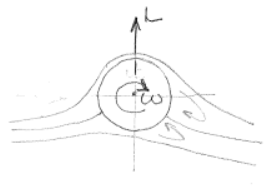
\includegraphics[width=0.3\linewidth]{Figures/liftingFlowOverCylinder.PNG}
    \caption{Lifting flow over a cylinder with circulation}
    \label{fig:LiftingFlowOverCulinder}
\end{figure}
Figure \ref{fig:LiftingFlowOverCulinder} shows a cylinder rotating at speed $\omega$. This produces a curved flight path like a baseball's.

\begin{figure}[ht]
    \centering
    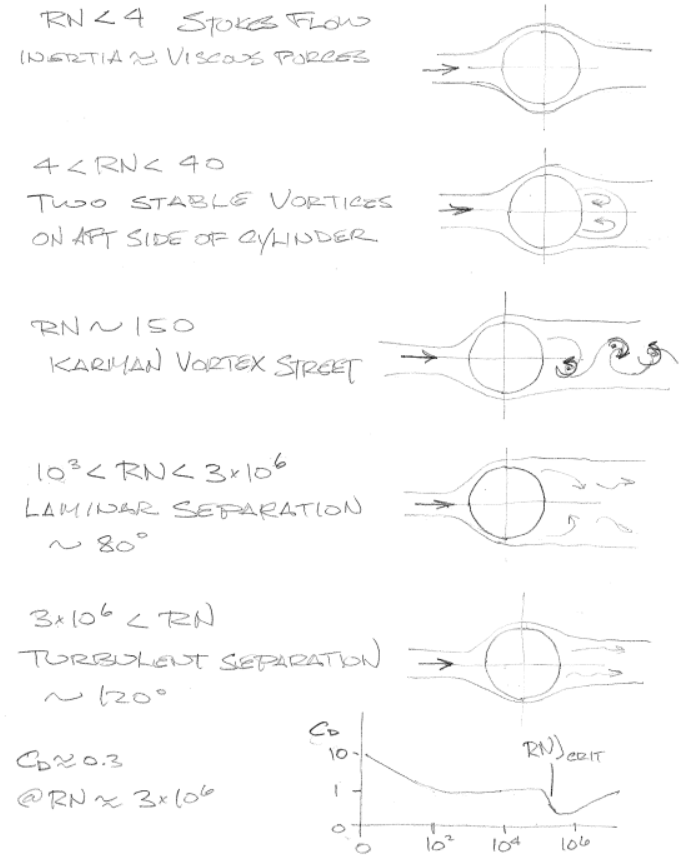
\includegraphics[width=0.7\linewidth]{Figures/realFlowOverCylinders.PNG}
    \caption{Real flow over cylinders at varying Reynolds numbers}
    \label{fig:RealFlowOverCylinders}
\end{figure}

% Liebeck: "I've never failed a graduating senior."
% Liebeck: "If I fail them, they're not graduating."

\subsection{Theory of Lift}
\begin{figure}[ht]
    \centering
    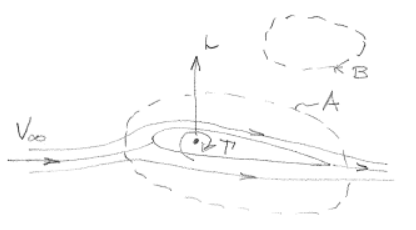
\includegraphics[width=0.4\linewidth]{Figures/circulationAroundAirfoil.PNG}
    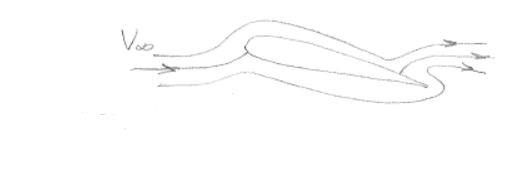
\includegraphics[width=0.5\linewidth]{Figures/liftingFlowOverAirfoil.PNG}
    \caption{Circulation around an airfoil and potential flow around an airfoil with $\Gamma=0$}
    \label{fig:CirculationFlowAirfoil}
\end{figure}
Recall circulation (Equation \ref{eq:Circulation}). Then in Figure \ref{fig:CirculationFlowAirfoil}:
\begin{equation*}
    \Gamma = \oint_A \vec{V} \bullet \vec{ds} \quad\text{and}\quad \oint_B \vec{V} \bullet \vec{ds} = 0
\end{equation*}
Figure \ref{fig:CirculationFlowAirfoil} shows a potential flow about an airfoil with $\Gamma=0$. Viscosity will not permit this flow about the trailing edge. Adding a vortex and setting its strength $\Gamma$ such that the flow passes smoothly off the trailing edge defines a streamline geometry that simulates the real flow. This value of $\Gamma$ also correctly predicts the lift from
\begin{equation*}
L = \rho V \Gamma
\end{equation*}

% PRAGMA MARK NEW SECTION page 76 Source Panel Method
\section{Source Panel Method}
\subsection{Point and Sheet Source}
\begin{figure}[ht]
    \centering
    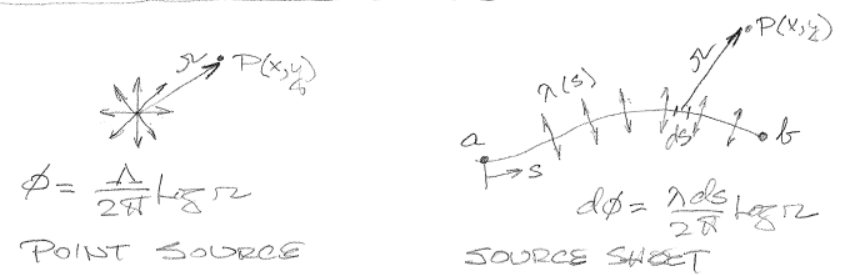
\includegraphics[width=0.9\linewidth]{Figures/pointAndSheetSource.PNG}
    \caption{Point source and source sheet}
    \label{fig:pointAndSheetSource}
\end{figure}
For a source sheet of varying strength $\lambda (s)$, apply Equation \ref{eq:sourceSheetStrength} (Figure \ref{fig:pointAndSheetSource}).
\begin{equation}
    \Phi(x,y) = \int_a^b \frac{\lambda(s)}{2\pi} ds \log(r)
    \label{eq:sourceSheetStrength}
\end{equation}
Source-panel method represents an arbitrary body by a series of flat panels, each with a constant source strength $\lambda_j$. Thus, the velocity potential induced at $P(x y)$ due to the $j^{th}$ panel is Equation \ref{eq:sourceSheetj} where the integral is over the $j^{th}$ panel (Figure \ref{fig:sourcePanelBody}).

\begin{figure}[ht]
    \centering
    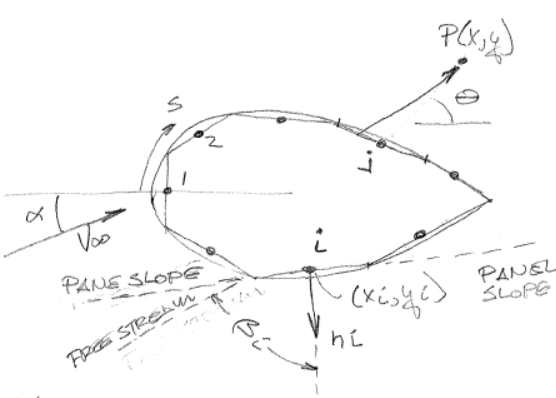
\includegraphics[width=0.5\linewidth]{Figures/sourcePanelBody.PNG}
    \caption{A body composed of source panels}
    \label{fig:sourcePanelBody}
\end{figure}
\begin{equation}
    \Delta \Phi_j = \frac{\lambda_j}{2\pi} \int_j \log(r_{pj})ds_j
    \label{eq:sourceSheetj}
\end{equation}

In turn, the velocity potential at P due to all of the panels is Equation \ref{eq:sourceSheetAllj}
\begin{equation}
    \Phi(P) =\sum_{j=1}^n \Delta \Phi_j = \sum_{j=1}^n \frac{\lambda_j}{2\pi} \int_j \log(r_{pj})ds_j
    \label{eq:sourceSheetAllj}
\end{equation}
where $r_{p1}$ is given by
\begin{equation*}
    r_{p1} = \sqrt{ (s-s_j)^2 + (y-y_j)^2 }
\end{equation*}

Next, select $P(x,y)$ to be $P(x_i, y_i)$, the \textbf{control point} of the $i^{th}$ panel. The boundary condition for the body to be a streamline is that the normal component of the velocity is zero. The free stream component normal to the $i^{th}$ panel is
\begin{equation*}
    V_{\infty, n} = V_\infty \bullet n_i = V_\infty \cos\beta_i
\end{equation*}
$V_\infty$ is positive away from the body.
\paragraph*{} The normal component of the velocity induced by the source panel is
\begin{equation*}
V_n= \partialfrac{}{n_i} \big[ \Phi(x_i, y_i) \big]
\end{equation*}
(Again, $V_n$ is positive away from the body.)\\

% If I write my panel code in C++ nobody can ask me to help them with their Matlab spaghetti

Note: When $j=i$ in the sum for $\Phi(P),\ r_{pj=i}=0$ which is a singularity. It can be shown that the contribution to $V_n$ is $\lambda_i/2$. Therefore, the expression for $V_n$ becomes
\begin{equation*}
    V_n = \frac{\lambda_i}{2} + \sum_{j=1,\ j\neq i}^n \frac{\lambda_i}{2\pi} \int_j \partialfrac{}{n_i} \log(r_{ij})ds_j
\end{equation*}
The boundary condition for flow tangency is
\begin{align*}
   &  V_{\infty n} + V_n = 0\\
    \text{or} \quad& \frac{\lambda_i}{2} + \sum_{j=1,\ j\neq i}^n \frac{\lambda_j}{2\pi} \int_j \partialfrac{}{n_i} \log(r_{ij}) ds_j + V_\infty \cos\beta_i = 0\\
    \text{Writing} \quad& I_{ij} = \int_j \partialfrac{}{n_i} \log(r_{ij} ds_j
\end{align*}
It is noted that $I_{ij}$ is a function of \textbf{panel geometry} alone, and it is not a function of the flow properties.
\begin{equation*}
    \text{Thus} \quad
    \frac{\lambda_i}{2} + \sum_{j=1,\ j\neq i}^n \frac{\lambda_j}{2\pi} I_{ij} + V_\infty \cos\beta_i = 0
\end{equation*}
is a set of n \textbf{linear algebraic equations} in the n unknowns $\lambda_j$. The solution for the source panel strengths $\lambda_j$ provides a flow where the body surface is a streamline.

% I could use CoCalc for the source panel code if I wrote in Python; then I could link the code and report.
\paragraph*{} The velocity \textbf{tangent} to the surface at the $i^{th}$ panel is given by
\begin{gather*}
    V_i = V_{\infty s} + V_s = V_\infty \sin\beta_i + \partialfrac{\Phi}{s}\\
    V_i = V_\infty\sin\beta_i + \sum_{j=1}^n \frac{\lambda_j}{2\pi} \int_j \partialfrac{}{s} \log(r_{ij}) ds_j
\end{gather*}

(Here, the contribution of the $i^{th}$ source panel to the tangential velocity there is by definition zero.)
\paragraph*{}
Once $V_i$ on the body surface is known, the corresponding pressure coefficient is simply
\begin{equation*}
    C_{pi} = 1-\Big(\frac{V_i}{V_\infty}\Big)^2
\end{equation*}
And thus the pressure distribution over a non-lifting body of arbitrary geometry can be calculated.\\
As a check, for a closed body, the sum of the source(sink) strengths must be zero (Equation \ref{eq:sourcePanelCheck}).
\begin{equation}
    \sum_{j=1}^n \lambda_j s_j = 0
    \label{eq:sourcePanelCheck}
\end{equation}

% But if I write in C++ I have a reason to learn openGL for plotting
\begin{figure}[ht]
    \centering
    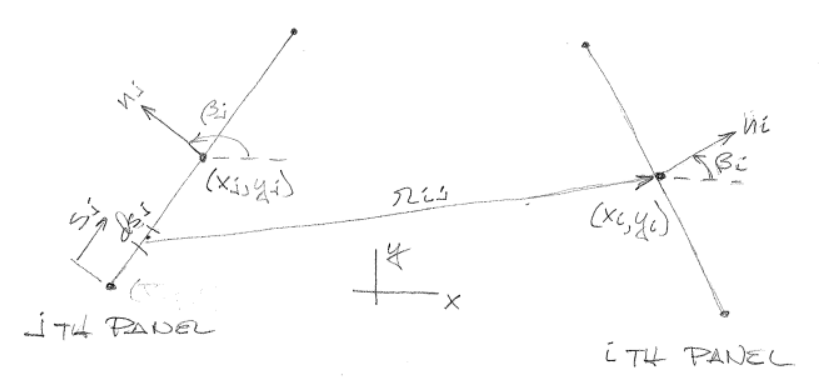
\includegraphics[width=0.8\linewidth]{Figures/sourcePanels2.PNG}
    \caption{Corresponding $i^{th}$ and $j^{th}$ panels}
    \label{fig:sourcePanels2}
\end{figure}
\begin{align*}
    I_{ij} &= \int_j \partialfrac{}{n_i} \big(\log r_{ij}\big) ds_j\\
    \partialfrac{}{n_i} \big(\log r_{ij}\big) &=
    \frac{1}{r_{ij}} \partialfrac{r_{ij}}{n_i}\\
    &=
    \frac{1}{r_{ij}}\frac{1}{2}\Big[ (x_i-x_j)^2 + (y_i-y_j)^2 \Big]^{-1/2} \cdot
    \Big[ 2(x_i-x_j)\frac{dx_i}{dn_i} + 2(y_i-y_j)\frac{dy_i}{du_i} \Big]\\
    \frac{dx_i}{du_i} &=
    \cos\beta_i,\quad \frac{dy_i}{du_i} = \sin\beta_i\\
    \partialfrac{}{u_i}\big( \log r_{ij} \big) &=
    \frac{ (x_i-x_j) \cos\beta_i + (y_i-y_j)\sin\beta_i }{ (x_i-x_j)^2 + (y_i-y_j)^2 }
\end{align*}
This must be integrated over $s_j$ to obtain a general expression for $I_{ij}$ for two arbitrary panels. See pages 225-227 in text.

% PRAGMA MARK NEW SECTION page 81 Airfoil Characteristics
\section{Airfoils}
\subsection{Airfoil Characteristics}
\begin{figure}[ht]
    \centering
    \includegraphics[width=0.7\linewidth]{Figures/airfoilCharacteristics.PNG}
    \caption{Characteristics of an airfoil and plots of $C_l,\ C_d,\ C_{M,ac}$}
    \label{fig:AirfoilCharacteristics}
\end{figure}
\begin{enumerate}
    \item In Figure \ref{fig:AirfoilCharacteristics}: Airfoil thickness relates to structure and the range of $\alpha$
    \item Camber relates to the designed $C_l,\ \alpha_{ol}$ and designed $\alpha$
    \item Aerodynamic center: $C_m$ is invariant with respect to $C_l$ near $C/4$.
    \item Reynolds Number: Increasing $RN = \frac{\rho V c}{\mu}$ increases $C_{l,max}$ and decreases $C_d$
\end{enumerate}
\begin{figure}[ht]
    \centering
    \includegraphics[width=0.6\linewidth]{Figures/airfoilStallFlow.PNG}
    \caption{Attached flow and stall conditions on an airfoil}
    \label{fig:AirfoilStallFlow}
\end{figure}

\subsection{Vortex Sheet}
\begin{figure}[ht]
    \centering
    \includegraphics[width=0.6\linewidth]{Figures/vortexSheet.PNG}
    \caption{Airfoil surface as vortex sheet}
    \label{fig:VortexSheet}
\end{figure}
Define $\gamma(s)$ as the strength of the vortex sheet / unit length. Then the vortex strength is $\gamma ds$. Recall that for a point vortex, $V=-\Gamma/(2\pi r)$. Then the velocity induced at P by the vortex sheet element $ds$ is
\begin{equation*}
    dV = -\frac{\gamma ds}{2\pi r}
\end{equation*}
In this equation $dV$ is $\perp$ to $r$. If the $dV$'s in Figure \ref{fig:VortexSheet} are to be summed from a to b, they must be added vectorially. Therefore, use the velocity potential
\begin{align*}
    \Phi &= -\frac{\Gamma\theta}{2\pi} \rightarrow d\Phi = -\frac{\gamma ds}{2\pi}\theta\\
    \text{or} \quad \Phi(x,y) &= -\frac{\Gamma\theta}{2\pi} = -\frac{1}{2\pi}\int_a^b\theta\gamma ds
\end{align*}
The total circulation is Equation \ref{eq:VortexSheetCirculation}.
\begin{equation}
    \Gamma = \int_a^b\gamma ds
    \label{eq:VortexSheetCirculation}
\end{equation}

Recall for a \textbf{source sheet}, tangential V is continuous across the sheet. Normal V changes direction $180\degree$.\\
For a \textbf{vortex sheet}: tangential V is discontinuous across the sheet and normal V is continuous.
\begin{figure}[ht]
    \centering
    \includegraphics[width=0.3\linewidth]{Figures/vortexSheet2.PNG}
    \caption{A section of the vortex sheet with circulation}
    \label{fig:VortexSheet2}
\end{figure}

% Is anyone reading these?

In Figure \ref{fig:VortexSheet2}, consider a section of the vortex sheet $ds$ and the circulation $\Gamma$ about $ds$.
\begin{equation*}
    \Gamma = -v_2du + u_1ds + v_1du - u_2ds = (u_1-u_2)ds + (v_1-v_2)du
\end{equation*}
Let the top and bottom approach the sheet, i.e. $dn \rightarrow 0$
\begin{gather*}
    \lim\limits_{du \rightarrow 0} \Gamma = (u_1-u_2)ds\\
    \text{But also, } \Gamma = \gamma ds, \text{ therefore}\\
    \gamma = u_1-u_2
\end{gather*}
The local velocity jump across the sheet is equal to the strength.\\
Analogous to the source panel method, represent an airfoil by a vortex sheet over its surface. Set the variation of $\gamma(s)$ such that the airfoil shape becomes a streamline. Then
\begin{equation*}
    L = \rho_\infty V_\infty \Gamma = \rho_\infty V_\infty \int\gamma ds
\end{equation*}
\subsubsection{Thin Airfoil Approximation}
\begin{figure}[ht]
    \centering
    \includegraphics[width=0.7\linewidth]{Figures/thinAirfoilApproximation.PNG}
    \caption{Approximation of a real airfoil as a vortex sheet}
    \label{fig:ThinAirfoilApproximation}
\end{figure}
See Figure \ref{fig:ThinAirfoilApproximation}. \textbf{Camber} is the primary input to aerodynamic performance.

\subsubsection{Trailing Edge / Kutta Condition}
\begin{figure}[ht]
    \centering
    \includegraphics[width=0.7\linewidth]{Figures/trailingEdgeCondition.PNG}
    \caption{Flow at the trailing edge of the airfoil (Kutta Condition)}
    \label{fig:TrailingEdgeCondition}
\end{figure}
See Figure \ref{fig:TrailingEdgeCondition}. The Kutta condition is Equation \ref{eq:KuttaCondition}.
\begin{equation}
    \gamma(TE) = V_1-V_2 = 0
    \label{eq:KuttaCondition}
\end{equation}

\subsection{Vortex Theorem of Kelvin}
"The circulation around any path which is always made up of the same fluid particles is independent of the time."\\
"In a perfect fluid, no tangential forces can act, and hence the angular velocity of a fluid particle can never change since no couple can be exerted on it." -Clark Millikan
\begin{equation}
    \frac{D\Gamma}{dt} = 0
    \label{eq:KelvinVortexTheorem}
\end{equation}
\begin{figure}[ht]
    \centering
    \includegraphics[width=0.7\linewidth]{Figures/kelvinVortexTheorem.PNG}
    \caption{The starting vortex forms moments after the flow begins moving over the airfoil}
    \label{fig:StartingVortex}
\end{figure}

Figure \ref{fig:StartingVortex} shows that just as the airfoil starts to move, the high velocity gradient about the trailing edge forms a "starting vortex" that is swept downstream.
\begin{gather*}
    \frac{D\Gamma}{Dt} = 0 \rightarrow \Gamma_1 = \Gamma_2 = 0\\
    \Gamma_2 + \Gamma_4 = \Gamma_2 \ 0\\
    \rightarrow \Gamma_4 = -\Gamma_3
\end{gather*}
Once a steady state is reached, the starting vortex $\Gamma_3$ is swept far downstream, and steady flow with circulation $\Gamma_4$ about the airfoil is established.
% left off here for midterm, last page is 86

% the midterm is tomorrow
% and if you're reading this source maybe you think emi is some kind of, idk, smart student
% but I'm not, and I'm scared of the midterm
% and I did this anyway, so if you're wondering how one student did all this: one page at a time
% be the change you want to see
% -emi, November 4th 2018, 7:08 PM

\section{Thin Airfoil Theory}
\subsection{Vortex Sheet}
\begin{figure}[ht]
    \centering
    \includegraphics[width=0.8\linewidth]{Figures/vortexSheetOnLine.PNG}
    \caption{A vortex sheet on the camber line and a vortex sheet on the chord line}
    \label{fig:vortexSheetOnLine}
\end{figure}
Define the airfoil as a vortex sheet on the camber line (Figure \ref{fig:vortexSheetOnLine}). Move the vortex sheet to the chord line $\gamma(s) \rightarrow \gamma(x)$ and $\gamma (c) = 0$, but set the strength of the vortex sheet such that the camber line (not the chord line) is a streamline.
\begin{equation*}
    V_{\infty n} + w(s) = 0
\end{equation*}
$V_\infty n$ is the component of $V_\infty$ normal to the camber line. $w(s)$ is the velocity induced by the vortex sheet normal to the camber line (Figure \ref{fig:vortexSheetDifferential}).
\begin{gather*}
    V_{\infty n} = V_\infty \sin\big[ \alpha + \arctan(-\frac{dz}{dx})\big]\\
    \text{For small } \alpha \text{ and } dz/dx \quad V_{\infty n} = V_\infty \big[\alpha - \frac{dz}{dx}\big]
\end{gather*}
\begin{figure}[ht]
    \centering
    \includegraphics[width=0.4\linewidth]{Figures/vortexSheetDifferential.PNG}
    \caption{$V_{\infty n}$ on a vortex sheet}
    \label{fig:vortexSheetDifferential}
\end{figure}

A consistent approximation is $w(s) = w(x)$ where $w(x)$ is the component of velocity induced by the vortex sheet normal to the chord line (Figure \ref{fig:vortexSheetApproximation}).
\begin{figure}[ht]
    \centering
    \includegraphics[width=0.4\linewidth]{Figures/vortexSheetApproximation.PNG}
    \caption{Approximating $w(s) = w(x)$ for a vortex sheet}
    \label{fig:vortexSheetApproximation}
\end{figure}
\begin{align*}
    \gamma &= \gamma(\zeta)\\
    dw(x) &= -\frac{\gamma(\zeta) d\zeta}{2\pi (x-\zeta)}\\
    w(x) &= -\int_0^c \frac{\gamma(\zeta)d\zeta}{2\pi (x-\zeta)}\\
    \text{Recalling} \quad V_{\infty n} + w(s) = 0,&\quad V_{\infty n}= V_\infty(\alpha - dz/dx)
\end{align*}
\begin{equation}
        \frac{1}{2\pi}\int_0^c \frac{\gamma(\zeta)d\zeta}{x-\zeta} = V_\infty (\alpha - dz/dx)
        \label{eq:thinAirfoilEquation}
\end{equation}
% fundamental equation of thin airfoil theory
Equation \ref{eq:thinAirfoilEquation} is called the "Fundamental Equation of Thin Airfoil Theory" - it states that the camber line is a streamline.

% WE GET OUR MIDTERMS BACK TOMORROW
\subsection{Symmetric Airfoil}
For a symmetric airfoil, $dz/dx=0$ so 
\begin{equation}
    \frac{1}{2\pi}\int_0^c \frac{\gamma(\zeta)d\zeta}{x-\zeta} = V_\infty (\alpha)
    \label{eq:thinAirfoilEqSymmetric}
\end{equation}
Since thickness is not included, Equation \ref{eq:thinAirfoilEquation} becomes Equation \ref{eq:thinAirfoilEqSymmetric}. This is an exact expression for the inviscid, incompressible flow over a \textbf{flat plate} at angle of attack $\alpha$. To solve for $\gamma(\zeta)$:
\begin{align*}
    \text{Apply the transformation} \quad& \zeta = \frac{c}{2}(1-\cos\theta),\quad d\zeta = \frac{c}{2} \sin \theta d\theta\\
    \text{Let the fixed point x correspond to a particular }&\ \theta = \theta_0,\ x_0 = \frac{c}{2} (1-\cos\theta_0)\\
    \text{The limits on the integral become } \theta = 0,\ \theta = \pi \quad& \frac{1}{2\pi} \int_0^\pi \frac{\gamma(\theta)\sin\theta d\theta}{\cos\theta - \cos\theta_0} = V_\infty \alpha\\
    \text{The solution to this integral equation is given by} \quad& \gamma(\theta) = 2\alpha V_\infty \frac{1+\cos\theta}{\sin\theta}
\end{align*}

This can be checked by substitution
\begin{equation*}
    \frac{1}{2\pi} \int_0^\pi \frac{\gamma(\theta)\sin\theta d\theta}{\cos\theta - \cos\theta_0} = \frac{V_\infty \alpha}{\pi} \int_0^\pi \frac{(1+\cos\theta)d\theta}{\cos\theta - \cos\theta_0}
\end{equation*}
And using the integral result
\begin{gather*}
    \frac{1}{2\pi} \int_0^\pi \frac{\cos u\theta d\theta}{\cos\theta - \cos\theta_0)} = \frac{\pi \sin u\theta_0}{\sin\theta_0}\\
    \frac{V_\infty \alpha}{\pi} \int_0^\pi \frac{(1+\cos \theta)d\theta}{\cos\theta - \cos\theta_0} = \frac{V_\infty \alpha}{\pi} \big( 0 + \pi \big) = V_\infty \alpha
\end{gather*}

The trailing edge condition $\gamma(\pi) = 0$ must be evaluated using L'Hopital's Rule:
\begin{equation*}
    \gamma(\pi) = 2\alpha V_\infty \frac{1-\cos\pi}{\sin \pi} = 2\alpha V_\infty \frac{-\sin\pi}{\cos\pi} = 0
\end{equation*}
The total circulation about the airfoil is
\begin{gather*}
    \Gamma = \int_0^c \gamma(\zeta) d\zeta = \frac{c}{2} \int_0^\pi \gamma(\theta)\sin\theta d\theta\\
    \Gamma = \alpha c V_\infty \int_0^\pi \big(1 + \cos\theta \big) d\theta = \pi \alpha c V_\infty\\
    \text{and the lift is} \quad L = \rho_\infty V_\infty \Gamma = \pi \alpha c \rho_\infty V_\infty^2\\
    C_l = \frac{L}{\frac{1}{2}\rho_\infty V_\infty^2 c} = \frac{\pi \alpha c \rho_\infty V_\infty^2}{\frac{1}{2} \rho_\infty V_\infty^2 c} = 2\pi \alpha,\quad \boxed{\frac{dc_l}{d\alpha} = 2\pi}
\end{gather*}
% End of Page 90
The moment about the leading edge (Figure \ref{fig:momentLeadingEdge}) is
\begin{figure}[ht]
    \centering
    \includegraphics[width=0.4\linewidth]{Figures/momentLeadingEdgePg91.PNG}
    \caption{Moment about the leading edge of the wing}
    \label{fig:momentLeadingEdge}
\end{figure}

\begin{gather*}
    dM = -\zeta\ dL\\
    dL = \rho_\infty V_\infty\ d\Gamma\\
    dL = \rho_\infty V_\infty \gamma(\zeta)\ d\zeta\\
    M_{LE} = -\int_0^c \rho_\infty V_\infty \gamma(\zeta) \zeta\ d\zeta = -\rho)\infty V_\infty \int_0^c \zeta \lambda(\zeta)\ d\zeta
\end{gather*}
\begin{align*}
    \text{Transforming} \quad \zeta &= \frac{c}{2}\big(1-\cos\theta\big),\quad d\zeta = \frac{c}{2}\sin\theta\ d\theta\\
    M_{LE} &= -\rho_\infty V_\infty \frac{c^2}{4} \int_0^\pi \gamma(\theta)(1-\cos\theta) \sin\theta\ d\theta\\
    \gamma(\theta) &= 2\alpha V_\infty \frac{1+\cos\theta}{\sin\theta}\\
    M_{LE} &= -\frac{1}{2} \rho_\infty V_\infty^2 c^2\alpha \int_0^\pi (1-\cos^2\theta) d\theta\\
    M_{LE} &= -q_\infty c^2 \alpha\pi/2\\
    C_{M,LE} &= \frac{M_{LE}}{q_\infty c^2} = -\frac{\pi}{2}\alpha\\
    \text{Using} \quad c_l &= 2\pi \alpha \rightarrow C_{M,LE} = -c_l/4\\
    \text{Recalling} \quad C_{M,LE} &= -c_l/4 + C_{M,ac/4},\quad \text{then } \boxed{C_{M,c/4} = 0}
\end{align*}

% MAYBE I SHOULD BE STUDYING FOR CS 143A
\subsection{Cambered Airfoil}
Recall
\begin{equation*}
    \frac{1}{2\pi} \int_0^c \frac{\gamma(\zeta)\ d\zeta}{x-\zeta} = V_\infty \Big( \alpha - \frac{dz}{dx}\Big)
\end{equation*}
where $dz/dx \neq 0$ and is a function of x. Again, transform to $\theta$:
\begin{equation*}
    \frac{1}{2\pi} \int_0^\pi \frac{\gamma(\theta)\sin\theta\ d\theta}{\cos\theta - \cos\theta_0} = V_\infty \Big(\alpha - \frac{dz}{dx}\Big)
\end{equation*}

$\gamma(\theta)$ where $\gamma(\pi) = 0$ will provide a solution where the camber line is a streamline. Here, the solution to the integral equation is:
\begin{equation*}
    \gamma(\theta) = 2 V_\infty \Bigg( A_0 \frac{1+\cos\theta}{\sin\theta} + \sum_{n=1}^\infty A_n \sin n\theta\Bigg)
\end{equation*}
The first term is similar to the symmetric case, and the rest is a Fourier series. $A_0$ and the $A_n$ depend on $dz/dx,\ \alpha$.\\
Substituting this solution:
\begin{equation*}
    \frac{1}{\pi} \int_0^\pi \frac{A_0 (1+\cos\theta) d\theta}{\cos\theta - \cos\theta_0} + \frac{1}{\pi} \sum_{n=1}^\infty \int_0^\pi \frac{A_n \sin n\theta \sin\theta\ d\theta}{\cos\theta - \cos\theta_0} = \alpha -\frac{dz}{dx}
\end{equation*}
This first term is evaluated as in the symmetric case, and the $A_n$ terms use
\begin{equation*}
    \int_0^\pi \frac{\sin n\theta \sin\theta d\theta}{\cos\theta - \cos\theta_0} = -\pi \cos n\theta_0
\end{equation*}

This yields
\begin{gather*}
    A_0 - \sum_{n=1}^\infty A_n \cos n \theta_o = \alpha - \frac{dz}{dx}\\
    \text{or,} \quad \frac{dz}{dx} = (\alpha - A_0) + \sum_{n=1}^\infty A_n \cos n\theta_0
\end{gather*}
Note: $dz/dx$ is the slope of the camber line at $x=\frac{c}{2}(1-\cos\theta_0)$. The coefficients of the Fourier cosine series are obtained from
\begin{gather*}
    \alpha - A_0 = \frac{1}{\pi} \int_0^\pi \frac{dz}{dx}\ d\theta_0\\
    A_n = \frac{2}{\pi} \int_0^\pi \frac{dz}{dx} \cos n\theta_0\ d\theta_0
\end{gather*}
where $dz/dx$ is a function of $\theta_0$ from $0 \rightarrow \pi$, or $0 \rightarrow c$.
\begin{itemize}
    \item $A_0$ depends on $\alpha, dz/dx$, while the $A_n$ depend only on $dz/dx$.
    \item Note that $\gamma(\pi) = 0$ is satisfied and that when $dz/dx=0,\ \gamma(\theta)$ reduces to the symmetric case.
\end{itemize}

% "I was [something else] instead of studying. Story of my life." ~ not emi, but could have been
Solutions for $c_l$ and $c_m$:
\begin{align*}
    \Gamma &= \int_0^c \gamma(\zeta)\ d\zeta = \frac{c}{2} \int_0^\pi \gamma(\theta)\sin\theta\ d\theta\\
    \Gamma &= cV_\infty \Big[ A_0 \int_0^\pi (1+\cos\theta)d\theta + \sum_{n=1}^\infty A_n \int_0^\pi \sin n\theta \sin\theta\ d\theta \Big]\\
    \int_0^\pi (1+\cos\theta) d\theta = \pi,&\quad \int_0^\pi \sin^2\theta = \pi/2,\quad \int_0^\pi \sin n\theta \sin\theta\ d\theta = 0\ n \neq 1\\
    \Gamma &= cV_\infty \big( \pi A_0 + \frac{\pi}{2}A_1\big)\\
    L &= \rho_\infty V_\infty \Gamma = \frac{1}{2}\rho_\infty V_\infty^2 c \pi (2A_0 + A_1)\\
    c_l &= \pi (2A_0 + A_1)
\end{align*}

Substituting for $A_0,\ A_1$
\begin{equation*}
    c_l = 2\pi \Big[ \alpha + \frac{1}{\pi} \int_0^\pi \frac{dz}{dx}(\cos\theta_0 - 1) d\theta_0\Big]
\end{equation*}
\begin{align*}
    \text{Again} &\quad \frac{dc_l}{d\alpha} = 2\pi\\
    \text{Write} &\quad c_l = \frac{dc_l}{d\alpha}(\alpha - \alpha_{OL}) = 2\pi (\alpha - \alpha_{OL})\\
    \text{Where} &\quad \alpha_{OL} = -\frac{1}{\pi} \int_0^\pi \frac{dz}{dx}(\cos\theta_0 - 1) d\theta_0
\end{align*}

For $C_{M,LE}$ recall
\begin{align*}
    M_{LE} &= -\rho_\infty V_\infty\int_0^c \zeta x(\zeta)\ d\zeta\\
    M_{LE} &= -\frac{\rho_\infty V_\infty c^2}{4}\int_0^c(1-\cos\theta)\sin\theta \gamma(\theta)\ d\theta\\
    \text{or}\quad C_{M,LE} &= -\frac{1}{2 V_\infty} \int_0^c \gamma(\theta) (1-\cos\theta)\sin\theta\ d\theta\\
    \text{Substituting} \quad \gamma(\theta) &= 2V_\infty \Big[ A_0 \frac{1+\cos\theta}{\sin\theta} + \sum_{u=1}^\infty A_n\sin n\theta \Big]\\
    \text{and evaluating} \quad & \int_0^\pi \sin n \theta \sin \theta\ d\theta \text{ etc}\\
    \text{yields} \quad C_{M,LE} &= -\frac{\pi}{2} \Big( A_0 + A_1 - \frac{A_2}{2} \Big)\\
    \text{Subsituting} \quad c_l &= \pi(2A_0 - A_2) \quad \text{yields}\\
    C_{M,LE} &= -\Big[ \frac{c_l}{4} + \frac{\pi}{4} (A_1-A_2) \Big]
\end{align*}
Again, recalling $C_{M,LE} = -c_l/4 + C_{M,c/4}$ yields
\begin{equation*}
    C_{M,c/4} = \frac{\pi}{4} (A_2-A_1)
\end{equation*}
Since $A_1,\ A_2$ depend on camber but not $\alpha,\ C_{M,c/4}$ is invariant with $\alpha$.
\begin{equation*}
    \frac{X_{CP}}{c} = -\frac{C_{M,LE}}{c_l} = \frac{c}{4}\Big[ 1 + \frac{\pi}{c_l}(A_1-A_2) \Big]
\end{equation*}
% Update: I should have studied more for CS 143A

\subsection{Vortex Panel Method} is analogous to the source panel method (Figure \ref{fig:vortexPanelAirfoil}).
\begin{figure}[ht]
    \centering
    \includegraphics[width=0.4\linewidth]{Figures/vortexPanelAirfoil.PNG}
    \caption{Airfoil with vortex panels}
    \label{fig:vortexPanelAirfoil}
\end{figure}
\begin{itemize}
    \item Represents a body with panels of constant vortex strength $\gamma_i$/unit length.
    \item Seeks the set $\gamma_i,\ i=1\rightarrow n$ such that the body surface is a streamline.
    \item Can be applied directly to cases with \textbf{lift}.
\end{itemize}
The velocity potential $\Delta \Phi(x,y)$ induced by the vortex panel $j$ is given by
\begin{equation*}
    \Delta \Phi_k(x,y) = -\frac{1}{2\pi}\int_j \theta_{Pj} X_j ds_j
\end{equation*}
Where the integral is over the $j^{th}$ panel. The total velocity potential at P from all panels is Equation \ref{eq:vortexPanelTotalPhi}.
\begin{equation}
    \Phi(x,y) = \sum_{j-1}^n \Phi_j = -\sum_{j-1}^n \frac{\gamma_i}{2\pi} \int_j \theta_{Pj} ds_j
    \label{eq:vortexPanelTotalPhi}
\end{equation}
where \begin{equation*}
    \theta_{pj} = \arctan\big(\frac{y-y_j}{x-x_j}\big)
\end{equation*}
Next, P is located at the control point $(x_i, y_i)$ of the $i^{th}$ panel. 

% An airplane is a device that almost doesn't work. A helicopter is a device that almost does; luckily it's so ugly the Earth repels it. ~Liebeck
The velocity potential at $(x_i, y_i)$ is
\begin{gather*}
    \Phi(x_i, y+i) = -\sum_{j=1}^n \frac{\gamma_j}{2\pi} \int_j \theta_{ij} ds_j\\
    \text{Where} \quad \theta_{ij} = \arctan\big( \frac{y_i-y_j}{x_i-x_j} \big)
\end{gather*}
For the body to be a streamline, the normal velocity on each panel must = 0. The normal velocity induced by the vortex panels is:

\begin{align*}
    V_n (x_i, y_i) &= \partialfrac{}{n_i} \Big[ \Phi(x_i, y_i) \Big]\\
    &= -\sum_{j=1}^n \frac{\gamma_j}{2\pi} \int_j \partialfrac{\theta_{ij}}{n_i} ds_j
\end{align*}
And again the normal velocity of the freestream is
\begin{equation*}
    V_{\infty n} \ V_{infty} \cos\beta_i
\end{equation*}
The boundary condition becomes
\begin{gather*}
    V_{\infty n} + V_n = 0\\
    \text{or} \quad V_\infty \cos\beta_i - \sum_{j=1}^n \frac{\gamma_j}{2\pi} \int_j \partialfrac{}{n_i} \theta_{ij} ds_j\\
    \text{Defining} \quad I_{ij} = \int_j \partialfrac{\theta_{ij}}{n_j}ds_j
\end{gather*}

These integrals are functions of the body (panel) geometry alone. Thus:
\begin{equation*}
    V_\infty \cos\beta_i - \sum_{j=1}^u \frac{\gamma_i}{2\pi} I_{ij} = 0
\end{equation*}
is a set of u linear algebraic equations that can be solved for the u unknown vortex strengths $\gamma_j$.
\paragraph*{} Since the vortex panels by definition provide circulation, lift can result. This implies that the \textbf{Kutta Condition} must be satisfied at the trailing edge, as in Figure \ref{fig:vortexPanelTrailingEdge}: $\gamma(TE) = 0$.

\begin{figure}[ht]
    \centering
    \includegraphics[width=0.3\linewidth]{Figures/vortexPanelTrailingEdge.PNG}
    \includegraphics[width=0.3\linewidth]{Figures/vortexPanelTiny.PNG}
    \caption{Trailing edge of airfoil with Kutta Condition}
    \label{fig:vortexPanelTrailingEdge}
\end{figure}

% The average on Liebeck's midterm was 60%; yikes -emi
\paragraph*{} To approximate numerically, set $\gamma_i + \gamma_{i-1}=0$. Applying this gives $n+1$ equations for n unknowns, an overdetermined system. This is accommodated by not applying the flow tangency condition at one of the control points, and thus removing one of the u tangency equations. The remaining $n-1$ equations plus the Kutta condition equation now make up the set of n equations for the n unknowns $\gamma_i$.
\paragraph*{} To calculate the resulting tangential velocity, recall the condition for the velocity next to a vortex sheet: $\gamma = u_1-u_2$. Inside the body, set the velocity to zero then $\gamma = u_1 - 0 = u_1$. Thus the velocity tangent to the body is equal to the local vortex strength $\gamma_i$. The total circulation is Equation \ref{eq:vortexSheetCirculation}.
\begin{equation}
    \Gamma = \sum_{j=1}^n \gamma_j s_j
    \label{eq:vortexSheetCirculation}
\end{equation}
And the lift is Equation \ref{eq:vortexSheetLift}
\begin{equation}
    L = \rho_\infty V_\infty \sum_{j-1}^n \gamma_j s_j
    \label{eq:vortexSheetLift}
\end{equation}

\subsection{Real Airfoils}
See Figure \ref{fig:realAirfoils}.
\begin{figure}[ht]
    \centering
    \includegraphics[width=0.9\linewidth]{Figures/realAirfoils.PNG}
    \caption{$c_l$ for real airfoils with flaps and slats}
    \label{fig:realAirfoils}
\end{figure}

\subsection{Viscous Flow - Airfoil Drag}
Laminar boundary layer:
\begin{align*}
    \delta = \frac{5x}{\sqrt{RN_x}},&\quad RN_x = \frac{\rho_\infty V_\infty x}{\mu}\\
    \rightarrow \delta N\sqrt{x} &\quad c_f = \frac{1.328}{\sqrt{RN_x}}
\end{align*}
Turbulent boundary layer:
\begin{gather*}
    \delta = \frac{0.37x}{(RN_x)^{1/5}} \quad c_f = \frac{0.074}{(RN_c)^{1/5}}\\
    \text{where} \quad c_f = \frac{\tau}{\frac{1}{2}\rho_\infty V_\infty^2}
\end{gather*}
For \textbf{one side} of a flat plate: $c_f = c_d$

\clearpage % force large airfoil figure to stay in place

% PRAGMA MARK NEW SECTION page 102 WINGS
\section{Wings}
\subsection{Finite Wings}
\begin{figure}[ht]
    \centering
    \includegraphics[width=0.8\linewidth]{Figures/finiteWingStreamlines.PNG}
    \caption{Streamlines and tip vortices over a finite wing}
    \label{fig:finiteWingStreamlines}
\end{figure}
In Figure \ref{fig:finiteWingStreamlines}, the trailing vortices create a \textbf{downwash velocity} $w$ at the wing. This results in the local velocity at the wing being canted downward relative to the freestream velocity.

\begin{figure}[ht]
    \centering
    \includegraphics[width=0.8\linewidth]{Figures/effectiveAngle.PNG}
    \caption{Effective angle of attack vs real angle}
    \label{fig:effectiveAngle}
\end{figure}
Since the local lift is $\perp$ to the local velocity, the resulting cant of the lift vector creates \textbf{induced drag} $D_i$ (Figure \ref{fig:effectiveAngle}).

\subsection{Biot-Savart Law}
\begin{figure}[ht]
    \centering
    \includegraphics[width=0.4\linewidth]{Figures/vortexFilamentLine.PNG}
    \caption{Biot-Savart Law applied to a vortex filament line}
    \label{fig:vortexFilamentLine}
\end{figure}
Consider a vortex filament in space (Figure \ref{fig:vortexFilamentLine}) of strength $\Gamma$ - The segment $\vec{dl}$ induces a velocity at P given by Equation \ref{eq:biotSavartLaw}.
\begin{equation}
    \vec{dV} = \frac{\Gamma}{4\pi} \frac{\vec{dl}\times\vec{r}}{|\vec{r}|^2}
    \label{eq:biotSavartLaw}
\end{equation}
For a straight filament of infinite length, Equation \ref{eq:biotSavartLaw} becomes:
\begin{equation*}
    \vec{V} = \int_{-\infty}^\infty \frac{\Gamma}{4\pi} \frac{\vec{dl}\times\vec{r}}{|\vec{r}|^3}
\end{equation*}
Here, $\vec{dl}\times\vec{r} = dl\cdot r \sin\theta$ and $\vec{V}$ is down.
\begin{equation*}
    V = \frac{\Gamma}{4\pi} \int_{-\infty}^\infty \frac{\sin\theta}{r^2}dl
\end{equation*}

Defining $h$ as the normal distance from P to the filament:
\begin{gather*}
    r = \frac{h}{\sin\theta},\quad l = \frac{h}{\tan\theta},\quad dl = -\frac{h}{\sin^2\theta}d\theta\\
    V = -\frac{\Gamma}{2\pi h} \int_\pi^0 \sin\theta\ d\theta = \frac{\Gamma}{2\pi h}
\end{gather*}
For a \textbf{semi-infinite} vortex filament, where the filament begins at the point A of the normal to P:
\begin{equation*}
    V = \frac{1}{2}\Big( \frac{\Gamma}{2\pi h} \Big)  = \frac{\Gamma}{4\pi h}
\end{equation*}

Heimholtz' Vortex Theorems:
\begin{enumerate}
    \item The strength of a vortex filament is constant along its length.
    \item A vortex filament cannot end in a fluid; it must extend to the boundaries of the fluid (possibly $\pm \infty$) or form a closed path.
\end{enumerate}

\begin{figure}[ht]
    \centering
    \includegraphics[width=0.4\linewidth]{Figures/liftOverWing.PNG}
    \caption{Lift distribution along span of real wing}
    \label{fig:liftOverWing}
\end{figure}
\subsubsection{General thoughts on a finite wing}
\begin{itemize}
    \item Lift will vary with spanwise location (Figure \ref{fig:liftOverWing})
    \item Lift = 0 at wingtips
    \item $L'(y) = \rho_\infty V_\infty \Gamma(y)$
    \item $\Gamma(y)$ will vary with y.
\end{itemize}


\subsection{Prandtl's Lifting Line Theory}
\begin{figure}[ht]
    \centering
    \includegraphics[width=0.8\linewidth]{Figures/prandtlLiftingLineP105.PNG}
    \caption{Prandtl's Lifting Line Theory for a wing}
    \label{fig:prandtlLiftingLineP105}
\end{figure}
From the Biot-Savart Law:
\begin{equation*}
w(y) = -\frac{\Gamma}{4\pi (b/2 + y)} - \frac{\Gamma}{4\pi(b/2-y)} = -\frac{\Gamma}{4\pi}\frac{b}{(b/2)^2-y^2}
\end{equation*}
which shows that $w(y) \rightarrow \infty$ at $y=\pm b/2$ (Figure \ref{fig:prandtlLiftingLineP105}). Next, consider a finite number of horseshoe vortices superimposed along the lifting line (Figure \ref{fig:prandtlLiftingLine2P105}).
\begin{figure}[ht]
    \centering
    \includegraphics[width=0.8\linewidth]{Figures/prandtlLiftingLine2P105.PNG}
    \caption{Horseshoe vortices superimposed along Prandtl's lifting line}
    \label{fig:prandtlLiftingLine2P105}
\end{figure}
\begin{equation}
dw(y_0) = -\frac{(d\Gamma/dy)dy}{4\pi (y-y_0)}
    \label{eq:prandtlLiftingLine}
\end{equation}
Note: $d\Gamma/dy$ is negative since $\Gamma$ is decreasing as $y$ increases toward the wingtip. However $w$ is positive up for the sketch. Therefore Equation \ref{eq:prandtlLiftingLine} for $dw$ requires the minus sign.

\paragraph*{} The total velocity $w(y_0)$ is obtained by integrating over the entire trailing vortex sheet:
\begin{equation*}
    w(y_0) = -\frac{1}{4\pi} \int_{-b/2}^{b/2} \frac{(d\Gamma/dy)}{y-y_0}dy
\end{equation*}
The induced angle of attack at the spanwise station $y_0$ is Equation \ref{eq:inducedAOA}.
\begin{gather}
    \alpha_i(y_0) = \arctan \Big( -\frac{w(y_0)}{V_\infty} \Big) = -\frac{w(y_0)}{V_\infty} \quad \text{small angle}\\
    \text{or} \quad \alpha_i(y_0) = \frac{1}{4\pi V_\infty} \int_{-b/2}^{b/2} \frac{(d\Gamma/dy)}{y-y_0}dy
    \label{eq:inducedAOA}
\end{gather}

The lift coefficient of the airfoil at $y_0$ is:
\begin{gather*}
    c_l = a_0 \big[ \alpha_{EFF} (y_0) - \alpha_{OL} \big] = 2\pi \big[ \alpha_{EFF} (y_0) - \alpha_{OL}\big]\\
    \text{Also} \quad L = \frac{1}{2}\rho_\infty V_\infty^2 c(y_0)c_l = \rho_\infty V_\infty \Gamma(y_0)\\
    \text{or} \quad c_l = \frac{2\Gamma(y_0)}{V_\infty c(y_0)}
\end{gather*}
Combining and solving for $\alpha_{EFF}$, we get Equation \ref{eq:effectiveAOA}.
\begin{equation}
    \alpha_{EFF}(y_0) = \frac{\Gamma(y_0)}{\pi V_\infty c(y_0)} + \alpha_{OL}
    \label{eq:effectiveAOA}
\end{equation}
By definition, $\alpha_{EFF} = \alpha - \alpha_i$. Combining the expressions for $alpha_{EFF}$ (Equation \ref{eq:effectiveAOA}) and $\alpha_i$ (Equation \ref{eq:inducedAOA}), we get Equation \ref{eq:alphaPrandtlLiftingLine}, the \textbf{fundamental equation of Prandtl's Lifting Line Theory}.
\begin{equation}
    \alpha(y_0) = \frac{\Gamma(y_0)}{\pi V_\infty c(y_0)} + \alpha_{OL}(y_0) + \frac{1}{4\pi V_\infty} \int_{-b/2}^{b/2} \frac{(d\Gamma/dy)}{y-y_0}dy
    \label{eq:alphaPrandtlLiftingLine}
\end{equation}

Equation \ref{eq:alphaPrandtlLiftingLine} is an integral-differential equation with the unknown $\Gamma(y)$. For a given wing design, $\alpha,\ c,\ \alpha_{OL}$ and $V_\infty$ are known at each spanwise station. Solution of the fundamental equation yields $\Gamma(y)$ from $-b/2$ to $b/2$.
\paragraph*{} The lift distribution is obtained from:
\begin{equation*}
    L(y_0) = \rho_\infty V_\infty \Gamma(y_0)
\end{equation*}
The total lift is Equation \ref{eq:liftPrandtlLiftingLine}
\begin{gather}
    L = \rho_\infty V_\infty \int_{-b/2}^{b/2} \Gamma(y) dy\\
    c_L = \frac{L}{\frac{1}{2}\rho_\infty V_\infty^2 S} = \frac{2}{V_\infty S} \int_{-b/2}^{b/2} \Gamma(y) dy
    \label{eq:liftPrandtlLiftingLine}
\end{gather}
% end of page 107

Induced drag is given by Equation \ref{eq:inducedDrag}.
\begin{equation}
    D_i = L\sin\alpha_i = L\alpha_i \quad \text{for small angles}
    \label{eq:inducedDrag}
\end{equation}
Total induced drag is then:
\begin{gather*}
    D_i = \int_{-b/2}^{b/2} L(y) \alpha_i(y) dy = \rho_\infty V_\infty \int_{-b/2}^{b/2} \Gamma(y) \alpha_i(y) dy\\
    \text{and} \quad c_{Di} = \frac{Di}{\frac{1}{2}\rho_\infty V_\infty^2 S} = \frac{2}{V_\infty S} \int_{-b/2}^{b/2} \Gamma(y) \alpha_i(y) dy
\end{gather*}

% page 109
\subsubsection{Notes on Fundamental Equation of Lifting Line Theory}
\begin{align*}
    c_l &= 2\pi (\alpha_{EFF} - \alpha_{OL})\\
    &= 2\pi (\alpha - \alpha_i - \alpha_{OL})\\
    \alpha &= \frac{c_l}{2\pi} + \alpha_{OL} + \alpha_i\\
    L &= \frac{1}{2}\rho_\infty V_\infty^2 c(y_0) c_l(y_0) = \rho_\infty V_\infty \Gamma(y_0)\\
    &\rightarrow c_l(y_0) = \frac{2\Gamma(y_0)}{V_\infty c(y_0)}\\
    \alpha_i(y_0) &= \frac{1}{4\pi V_\infty} \int_{-b/2}^{b/2} \frac{(d\Gamma/dy)}{y_0-y}dy
\end{align*}
\begin{equation*}
    \alpha(y_0) = \frac{\Gamma(y_0)}{\pi V_\infty c(y_0)} + \alpha_{OL}(y_0) + \frac{1}{4\pi V_\infty} \int_{-b/2}^{b/2} \frac{(d\Gamma/dy)}{y_0-y}dy
\end{equation*}

\subsection{Elliptic Lift Distribution}
Assume an elliptic circulation distribution given by Equation \ref{eq:ellipticCirculation}
\begin{equation}
    \Gamma(y) = \Gamma_0 \sqrt{1-4\Big( \frac{y}{b}\Big)^2}
    \label{eq:ellipticCirculation}
\end{equation}
\begin{enumerate}
    \item $\Gamma_0$ is the circulation at midspan.
    \item $L(y) = \rho_\infty V_\infty \Gamma(y)$ is the elliptic lift distribution.
    \item $\Gamma(b/2) = \Gamma(-b/2) = 0$
\end{enumerate}
Note: This $\Gamma(y)$ has not been obtained as a direct solution of the fundamental equation. At this point, it is simply specified.
\paragraph*{} Calculation of Downwash:
\begin{gather*}
    \frac{d\Gamma}{dy} = -\frac{4\Gamma_0 y}{b^2 \big[ 1-4(y/b)^2 \big]^{1/2}}\\
    w(y_0) = -\frac{1}{4\pi} \int_{-b/2}^{b/2} \frac{(d\Gamma/dy)}{y-y_0}dy = \frac{\Gamma_0}{\pi b^2} \int_{-b/2}^{b/2} \frac{y}{\big[ 1-4(y/b)^2 \big]^{1/2} (y_0-y)}dy\\
    \text{Transform via} \quad y = \frac{b}{2}\cos\theta,\quad dy = -\frac{b}{2}\sin\theta\ d\theta\\
    \rightarrow w(\theta_0) = -\frac{\Gamma_0}{2\pi b} \int_0^\pi \frac{\cos\theta\ d\theta}{\cos\theta - \cos\theta_0} = -\frac{\Gamma_0}{2b}
\end{gather*}
\textbf{The downwash is constant} for an elliptic lift distribution. Also:
\begin{equation*}
    \alpha_i(y_0) = -\frac{w(y_0)}{V_\infty} = -\frac{\Gamma_0}{2bV_\infty} \quad \text{constant}
\end{equation*}
Note: $w$ and $\alpha_i \rightarrow 0$ as $b\rightarrow \infty$ (2D flow). For the total lift:
\begin{gather*}
    L = \rho_\infty V_\infty \Gamma_0 \int_{-b/2}^{b/2} \sqrt{1-4\Big(\frac{y}{b}\Big)^2} dy = \rho_\infty V_\infty \Gamma_0 \frac{b}{2} \int_0^\pi \sin^2\theta\ d\theta\\
    \rightarrow  L = \rho_\infty V_\infty \Gamma_0 \frac{b}{4}\pi\\
    \text{or} \quad \Gamma_0 = \frac{4L}{\rho_\infty V_\infty b\pi}\\
    \text{Using} \quad L = \frac{1}{2}\rho_\infty V_\infty^2 Sc_L \quad \text{yields}\\
    \Gamma_0 = \frac{2 V_\infty S c_L}{b\pi}\\
    \text{and} \quad \alpha_i \quad \text{becomes} \quad \alpha_i = \frac{Sc_L}{\pi b^2}\\
    \text{Define aspect ratio as} \quad AR = \frac{b^2}{S} \quad \text{then} \quad \alpha_i = \frac{c_L}{\pi AR}\\
    \text{Recall} \quad C_{Di} = \frac{2}{V_\infty S} \int_{-b/2}^{b/2}\Gamma(y) \alpha_i(y)dy\\
    C_{Di} = \frac{2\alpha c\Gamma_o b}{2V_\infty S}\int_0^\pi \sin^2\theta\ d\theta = \frac{\pi \alpha_i \Gamma_o b}{2V_\infty S}\\
    \text{or} \quad C_{D1} = \frac{\pi b}{2V_\infty S}\Big(\frac{C_L}{\pi R}\Big) \frac{2V_\infty SC_L}{b\pi}\\
    \boxed{C_{Di} = \frac{C_L^2}{\pi AR}}
\end{gather*}
% end of page 110

Consider a wing composed of the same airfoils with no geometric twist. It is desired to have an elliptic lift distribution.
\begin{align*}
    \text{No twist} & \rightarrow \alpha = const\\
    \text{Elliptic} & \rightarrow \alpha_i = const\\
    & \alpha_{EFF} = \alpha - \alpha_i = const\\
    \text{Common Airfoil} & \rightarrow \alpha_o,\ \alpha_{0L} = const\\
    & C_l = \alpha_o(\alpha_{EFF} - \alpha_{0L}) = const\\
    & L(y) = q_\infty c \cdot C_l\\
    & \rightarrow c(y) = \frac{L(y)}{q_\infty C_l} \quad \text{must vary elliptically}
\end{align*}
Few wings have elliptic planforms, however, the lift distribution on most wings is similar to elliptic.
\begin{equation*}
    C_{Di} = \frac{C_L^2}{\pi AR e},\quad 0.9 < e \le 1 \quad e=1 \ \text{Ellipse}
\end{equation*}

\subsection{Notes on Elliptic Lift Distribution}
The fundamental equation applies for an arbitrary wing geometry where $\alpha,\ \alpha_{0L}$ and $c$ are specified functions of $y$. In this case, $\Gamma(y)$ is the solution that is sought. However if $\Gamma(y)$ is specified, then the fundamental equation is reduced to a simple algebraic equation where the solution is $c(y)$.
\begin{align*}
    \text{For} \quad \Gamma(y) &= \Gamma_o \sqrt{1-4(y/b)^2}\\
    L(y) &= \rho_\infty V_\infty \Gamma_o \sqrt{1-4(y/b)^2} = C_l \frac{1}{2}\rho_\infty V_\infty^2 c\\
    \text{Then} \quad C_l c &= \frac{2\Gamma_o}{V_\infty} \sqrt{1-4(y/b)^2}
\end{align*}
This the product $C_l c$ must vary elliptically. For common airfoils and zero twist, this yields an elliptic planform.
\paragraph*{} However, $C_l$ intself could in principle provide the elliptic variation while $c=const$. Recall:
\begin{align*}
    C_l &= \alpha_0(\alpha - \alpha_{0L} - \alpha_i)\\
    \alpha &\rightarrow \text{Twist}\\
    \alpha_{0L} &\rightarrow \text{Camber}\\
    \alpha_i &= \text{Const for elliptic } \Gamma(y)
\end{align*}
% End of page 113

Thus $\alpha(y)$ and $\alpha_{0L}(y)$ could be set to provide (or at least contribute to) an elliptic $\Gamma(y)$ where $c(y)$ itself is not elliptic. In this case, if the angle of attack of the wing is changed, a constant $\Delta \alpha$ is added at \textbf{all} spanwise stations:
\begin{equation*}
    C_l = \alpha_0(\alpha + \Delta \alpha - \alpha_{0L} - \alpha_i)
\end{equation*}
and the product $C_l c$ will no longer vary elliptically.
\paragraph*{} However, for the special case of common airfoils with zero twist, the resulting $C_lc$ will remain elliptic at all angles of attack since $C_l = const$ and $c(y)$ is elliptic.
% End of page 114

\subsection{Shrenk Approximation}
Based on a comparison of experimental results, Shrenk showed the lift distribution on a non-elliptic planform with zero twist lies approximately halfway between that of an elliptic planform of the same area (Figure \ref{fig:shrenkApproximationPg115}).

\begin{figure}[ht]
    \centering
    \includegraphics[width=0.8\linewidth]{Figures/shrenkApproximationPg115.PNG}
    \caption{Shrenk approximation for a non-elliptic planform}
    \label{fig:shrenkApproximationPg115}
\end{figure}

\subsection{General Lift Distribution}
Consider the spanwise transformation:
\begin{equation*}
y = -\frac{b}{2}\cos\theta,\quad \theta = 0,\ y = -\frac{b}{2},\quad \theta = \pi,\ y = +\frac{b}{2}
\end{equation*}

The elliptic circulation distribution becomes
\begin{gather*}
    \Gamma(y) = \Gamma_o \Big[ 1-4\big(\frac{y}{b}\big)^2 \Big] ^{1/2} = \Gamma_o \Big[ 1-4\frac{b^2}{4}\frac{\cos^2\theta}{b^2} \Big]^{1/2}\\
    \text{or}\quad \Gamma(\theta) = \Gamma_o \sin\theta
\end{gather*}
For the general case, assume
\begin{gather*}
    \Gamma(\theta) = 2bV_\infty \sum_1^N A_n\sin n\theta\\
    \frac{d\Gamma}{dy} = \frac{d\Gamma}{d\theta}\frac{d\theta}{dy} = 2bV_\infty \sum_1^N n A_n \cos n\theta \frac{d\theta}{dy}
\end{gather*}
Substitute in the fundamental equation:
\begin{gather*}
    \alpha(\theta_0) = \frac{2b}{\pi c(\theta_0} \sum_1^N A_n \sin n\theta + \alpha_{0L} (\theta_0) + \frac{1}{\pi} \int_0^\pi \frac{\sum_1^N n A_n \cos n\theta}{\cos\theta - \cos\theta_0} d\theta\\
    \text{Recall}\quad \int_0^\pi \frac{\cos n\theta\ d\theta}{\cos\theta - \cos\theta_0} = \frac{\pi \sin n\theta}{\sin\theta_0}
\end{gather*}
The Fundamental Equation becomes Equation \ref{eq:fundamentalLiftDistribution}.
\begin{equation}
    \alpha(\theta_0) = \frac{2b}{\pi c(\theta_0)} \sum_1^N A_n \sin n\theta_0 + \alpha_{0L}(\theta_0) + \sum_1^N n A_n \frac{\sin n\theta_0}{\sin\theta_0}
    \label{eq:fundamentalLiftDistribution}
\end{equation}

$b,\ c(\theta_0)$ and $\alpha_{0L}(\theta_0)$ and the airfoil section properties are given by the geometry of the wing. Next select N representative spanwise stations $\theta_0$'s and write the fundamental equation for each. This yields N linear algebraic equations that can be solved for the N unknowns $A_1,\ A_2...A_n$.\\
This yields the circulation distribution $\Gamma(\theta_0)$.
\paragraph*{} For the lift coefficient:
\begin{gather*}
    C_L = \frac{2}{V_\infty S} \int_{-b/2}^{b/2} \Gamma(y)dy = \frac{2b^2}{S} \sum_1^N A_n \int_0^\pi \sin n\theta\ sin\theta\ d\theta\\
    \int_0^\pi \sin^2\theta\ d\theta = \frac{\pi}{2},\quad \int_0^\pi \sin n\theta\ \sin\theta\ d\theta = 0,\quad n>1\\
    \rightarrow C_L = A_1 \pi \frac{b^2}{S} = A_1 \pi AR
\end{gather*}

(Although $C_L$ depends on $A_1$ alone, allthe $A_n$'s must be solved for to obtain $A_1$.)
% End of page 117

\paragraph*{} For the induced drag coefficient:
\begin{align*}
    C_{Di} &= \frac{2}{V_\infty S} \int_{-b/2}^{b/2} \Gamma(y) \alpha_i(y) dy\\
    &= \frac{2b^2}{S} \int_0^\pi \big( \sum_1^N A_n \sin n\theta\big) \alpha_i (\theta) \sin n\theta\ d\theta\\
    \alpha_i(y_0) &= \frac{1}{4\pi V_\infty} \int_{-b/2}^{b/2} \frac{(d\Gamma/dy)}{y-y_0} dy = \frac{1}{\pi}\sum_1^N nA_n \int_0^\pi \frac{\cos u\theta}{\cos\theta - \cos\theta_0}d\theta\\
    \text{Then} \quad \alpha_i(\theta) &= \sum_1^N nA_n \frac{\sin n\theta}{\sin\theta}
\end{align*}
Substituting into the equation for $C_{DI}$:
\begin{equation*}
    C_{Di} = \frac{2b^2}{S} \int_0^\pi \big( \sum_1^N A_n \sin n\theta \big) \big( \sum_1^N n A_n \sin n\theta\big) d\theta
\end{equation*}
The integrand is a product of two summations whose terms have the form $\sin m\theta\ \sin k\theta$. However:
\begin{equation*}
    \int_0^\pi \sin m\theta\ \sin k\theta\ d\theta =
    \Big\{\begin{matrix} 0, & m\neq k\\ \pi/2, & m=k\\\end{matrix}
\end{equation*}
Thus $C_{Di}$ becomes
\begin{align*}
    C_{Di} &= \frac{2b^2}{S} \Big( \sum_1^N n A_n^2\Big) \frac{\pi}{2}= \pi AR \sum_1^N n A_n^2\\
    C_{Di} &= \pi AR \Big( A_1^2 + \sum_2^N nA_n^2\Big) - \pi AR A_1^2 \Big[ 1 + \sum_2^N \big(\frac{A_n}{A_1}\big)^2 \Big]
\end{align*}
% end of page 118

Recalling that $C_l \ A_1 \pi AR$:
\begin{equation*}
    C_{Di}  \frac{C_L^2}{\pi AR}(1+S), \quad S = \sum_2^N n\big(\ A_n/A_1\big)^2
\end{equation*}
Note: $A_1 > A_2 > ... A_N \ \rightarrow \ S$ is small. Also, $S \ge 0$.
\begin{equation*}
    \boxed{C_{Di} \ge \frac{C_L^2}{\pi AR} \rightarrow \text{Elliptic Distance provides minimum } C_{Di}}
\end{equation*}
The expression for $C_{Di}$ is typically Equation \ref{eq:Cdi}
\begin{equation}
    \boxed{C_{Di} = \frac{C_L^2}{\pi AR e},\quad e\le 1 \text{ is the span efficiency factor}}
    \label{eq:Cdi}
\end{equation}
% End of page 119

\subsection{Lift Curve Slope for a Finite Wing}
For a 2D Airfoil, $\alpha_0 = dC_l / d\alpha$. Define the lift curve slope for a finite wing as Equation \ref{eq:liftCurveSlopeFiniteWing}.
\begin{equation}
    \alpha = \frac{dC_L}{d\alpha}
    \label{eq:liftCurveSlopeFiniteWing}
\end{equation}
When a finite wing is at the geometric angle $\alpha$, it experiences a reduced angle $\alpha_{EFF}$ given by Equation \ref{eq:alphaEffFiniteWing}.(Figure \ref{fig:ellipticWingClPg120}).
\begin{equation}
    \alpha_{EFF} = \alpha - \alpha_i,\quad \text{where } \alpha_i = \frac{C_L}{\pi AR} \text{ (Elliptic)}
    \label{eq:alphaEffFiniteWing}
\end{equation}
\begin{figure}[ht]
    \centering
    \includegraphics[width=0.3\linewidth]{Figures/ellipticWingClPg120.PNG}
    \includegraphics[width=0.3\linewidth]{Figures/ellipticWingCl2Pg120.PNG}
    \caption{$C_L$ slope for $\alpha$ and $\alpha_{EFF}$. The slope $\alpha$ is less than $\alpha_0$}
    \label{fig:ellipticWingClPg120}
\end{figure}
Consider an elliptic wing with zero twist. Since $C_l = const$ across the span:
\begin{equation*}
    C_L = C_l
\end{equation*}
Since the wing experiences $\alpha_{EFF}$:
\begin{equation*}
    \frac{d C_L}{d\alpha_{EFF}} = \frac{d C_L}{d(\alpha - \alpha_i)} = \alpha_0
\end{equation*}
Integrating:
\begin{align*}
    C_L &= a_0(\alpha - \alpha_i) + const\\
    C_L &= a_0(\alpha - \frac{C_L}{\pi AR}) + const\\
    C_L \big(1+ \frac{a_o}{\pi AR}\big) = a_0 \alpha\\
    \frac{d C_L}{d\alpha} = a = \frac{a_0}{1+a_0/(\pi AR) (1+\tau)}
\end{align*}
% End of page 120

\subsection{Summary of Wing Drag}
Wing drag originates from 3 sources:
\begin{enumerate}
    \item $D_f$ due to skin friction
    \item $D_p$ due to separation (Pressure drag)
    \item $D_i$ due to lift
\end{enumerate}
Define $C_{DP} = \frac{D_f + D_p}{q_\infty S}$ as the profile drag coefficient. $C_{DP}$ is regarded as a function of the airfoil geometry and Reynolds Number, and is a weak function of $C_l$.
\begin{equation*}
    C_{Di} = \frac{D_i}{q\infty S} = \frac{C_L^2}{\pi AR e}
\end{equation*}
\begin{align*}
\text{Therefore total wing drag is} \quad&
    C_D = C_{DP} + \frac{D_L^2}{\pi AR e}\\
\text{For two of different aspect ratio:} \quad&
    C_{D_1} = C_{DP_1} + \frac{C_L^2}{\pi AR_1 e},\quad C_{D_2} = C_{DP_2} + \frac{D_L^2}{\pi AR_2 e}\\
\text{Assuming the same airfoil and twist:} \quad&
    C_{DP_1} = C_{DP_2} \quad \text{and} \quad e_1 = e_2 = e\\
\text{Taking the difference:} \quad&
    C_{D_1} - C_{D_2} = \frac{C_L^2}{\pi e} \big(\frac{1}{AR_1} - \frac{1}{AR_2}\big)
\end{align*}
% end of page 121

\begin{figure}[ht]
    \centering
    \includegraphics[width=0.8\linewidth]{Figures/dragPolarPg122.PNG}
    \caption{Drag polars for varying $AR$}
    \label{fig:dragPolarPg122}
\end{figure}
Using the relation:
\begin{equation*}
    C_{D_1} = C_{D_2} + \frac{C_L^2}{\pi e} \big( \frac{1}{6} + \frac{1}{AR_2}\big)
\end{equation*}
The data for $AR=4,\ 3$, etc. collapses onto the polar for $AR=6$ (Figure \ref{fig:dragPolarPg122}). Similarly, using the 3D lift curve slope definition (Equation \ref{eq:3DLiftCurveSlope}), the lift curve slopes collapse to a common curve in Figure \ref{fig:liftCurveSlopeCollapse}.

\begin{equation}
    a = \frac{a_0}{1+a_0/\pi AR) (1+\tau)}
    \label{eq:3DLiftCurveSlope}
\end{equation}
\begin{figure}[ht]
    \centering
    \includegraphics[width=0.3\linewidth]{Figures/dragPolar_ClPg122.PNG}
    \includegraphics[width=0.3\linewidth]{Figures/dragPolar_Cl2Pg122.PNG}
    \caption{The lift curve slopes collapse to a common curve for varying $AR$}
    \label{fig:liftCurveSlopeCollapse}
\end{figure}

$C_f = \tau /(\frac{1}{2}\rho V^2) = \tau/q$ and $D = \tau \times S_{wet}$ = drag force due to skin friction for a \textbf{flat plate} (Figure \ref{fig:dragFlatPlate}).

\begin{figure}[ht]
    \centering
    \includegraphics[width=0.3\linewidth]{Figures/dragFlatPlatePg123.PNG}
    \includegraphics[width=0.3\linewidth]{Figures/CfflatPlatePg123.PNG}
    \caption{Drag and $C_f$ on a flate plate}
    \label{fig:dragFlatPlate}
\end{figure}
% end of page 122

\begin{gather*}
    \text{Define } f = KC_f S_{wet} \ \text{as drag area}\\
    f = D/q\\
    C_D = \frac{D}{qS_{ref}} = \frac{f}{S_{ref}}\\
    \text{Then } f_{total} = \sum f_i = \sum K_i C_{fi} S_{wet,\ i}\\
    C_D = \frac{f_{total}}{S_{ref}}
\end{gather*}
% end of page 123

\begin{gather*}
\renewcommand{\arraystretch}{3.0}
    C_D = C_{DP} + C_{Di} = C_{DP} + \frac{C_L^2}{\pi AR e}\\
    D/L = C_D/C_L = \frac{C_{DP}}{C_L} + \frac{C_L}{\pi AR e}\\
    \frac{d(C_d/C_L)}{dC_L} = -\frac{C_{DP}}{C_L} + \frac{1}{\pi AR e} = 0\\
    C_{DP} = \frac{C_L^2}{\pi AR e} \text{ for } C_D/C_L\Big)_{min} \text{ or } C_L/C_D\Big)_{max}\\
    C_L\Big)_{L/D\ max} = \big( \pi AR e C_{DP}\big)^{1/2}\\
    \frac{C_L}{C_D}\big)_{max} = \frac{C_L}{C_{DP} + \frac{C_L^2}{\pi AR e}} =
    \frac{\big( \pi AR e C_{DP}\big)^{1/2}}{2C_{DP}} = \Big(\frac{\pi AR e}{4 C_{DP}}\Big)^{1/2}\\
    C_{DP} = \sum f_i/S_{ref} = \sum\frac{K_i C_{fi} S_{wet,\ i}}{S_{ref}} =
    \bar{K} \bar{C_f} \frac{S_{wet}}{S_{ref}}\\
    \frac{C_L}{C_D}\Big)_{max} = \Big(\frac{\pi b^2 e}{4 \bar{K} \bar{C_f} S_{wet}}\Big)^{1/2} =
    Big( \frac{\pi}{4} e \frac{b^2}{\bar{K}\bar{C_f} S_{wet}}\Big)^{1/2}\\
    \text{Optimum (max) lift:} \quad e=1,\ \bar{K}=1,\ C_f(RN)\\
    \text{Then} \quad L/D\Big)_{max} = \text{const}(AR_{wet})^{1/2}
\end{gather*}
% End of page 124!

\end{document}https://www.overleaf.com/project/5bc56340b43798777eed5b38